\chapter{COMPUTATIONAL METHODS: ION TRAJECTORY SIMULATIONS}
\markboth{COMPUTATIONAL METHODS}{}

Description of the computational model, experiments in DC and RF and comparison with the simulations for the reagent ions, which represent the majority of ions in the reactor.

Note this is only in the reactor and there are several more stages until the mass spectrometer which can influence the transmission of ions


\section{Introduction}

In the literature there are available some works, like for ESI with CFD \cite{doi:10.1002/jms.3519}. In the case of PTR-MS but with no scattering model \cite{ENNIS200572}

Ion funnels design parameters: see equation 7 in \cite{doi:10.1021/ac990346w}. Have a read at the whole article to refresh.


\section{Description of the model}









SIMION version ....

Montecarlo simulations

Collisional model HS1. Accounts for hard sphere collision. This model has been described in the literature \cite{appelhans2002measurement,DAHL20003,manura2008simion}. Briefly:
\begin{itemize}
\item The buffer gas is  neutral and its velocity follows the Maxwell-Boltzmann distribution\footnote[2]{From kinetic gas theory (Maxwell-Boltzmann), velocity in one dimension is normally distributed with standard deviation $\sigma_v = \sqrt{\frac{kT}{m}}$.}.
\end{itemize}


Collisions are assumed to be elastic as the only collisions accounted for are ion-neutral collisions, i.e. no proton transfer, clustering/declustering or fragmentation reactions are simulated.


The mean free path of the ions \cite{hirschfelder1954molecular}:
\begin{equation}
\label{eq:mfp}
\lambda = \frac{R T}{\sqrt{2} \pi d^2 N_A P} = \frac{k T}{\sqrt{2} \pi d^2 P}
\end{equation}
where R is the ideal gas constant, N$_A$ is Avogadro's number, T is the temperature, P is the pressure, d is the hard-sphere diameter of .... buffer gas? or sum of gas and ion?, 


\begin{figure}%[ht]
\centering
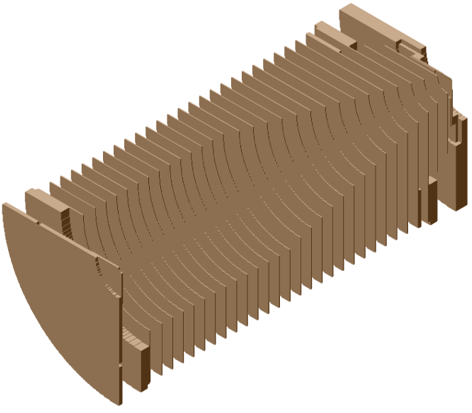
\includegraphics[width=0.7\linewidth]{pics/Reactor.PNG}
\centering
\caption{Geometry of the reactor used for the simulations in this chapter.}
\label{fig:sim_dt}
\end{figure}

\subsection{Parameters}

Table of parameters for SIMION are shown in table \ref{tb:sim}.

\begin{table}[ht]
\centering
\caption{List of parameters for the ion trajectory simulations.}
\label{tb:sim}
\begin{tabular}{lcc}
\toprule
\textbf{Parameter}	 &\textbf{Value}	&\textbf{Units} \quad\\ \midrule 
m/z           & 19, 37, 55, 73    	&Da?    				\\
ToB				& 	0.05				& $\mu$s\\
N				& 20000 			&ions \\
Coulombic Factor			&3$\times$10$^5$				&- \\
Drift voltage			&15-? 		&V \\
E/N (DC mode only)			&- 		&Td \\
Pressure			&1 				&mbar \\
Temperature			&100-150? 		&$^{\circ}$C \\
More parameters?? & & \\
\bottomrule
\end{tabular}
\end{table}

The time of birth (ToB) and the Coulombic factor are set to the values that yield a current of roughly 1 $\mu$A through the entry plate of the drift tube:
\begin{equation}
I = \frac{\Delta Q}{\Delta t} = \frac{3\times10^5 e}{0.05\, \mu s} = 0.96\, \mu A
\end{equation}



\subsection{Validation}
To validate the model and the parameters I compared the simulated results with the current measured at the exit plate with a picoammeter 








\section{Results and discussion}


\subsection{Drift time of ions in DC and RF mode}
Do some isolated ions flight at different voltages to measure drift times and compare to 1\slash V. Also to compare DC and RF modes. (N=1000, ungrouped)




 Files:
 \begin{itemize}
 \item DC mode: \verb|10-42-26_25-July-2018_simulation|
 \item RF mode: \verb|21-43-27_25-July-2018_simulation|
 \end{itemize}

 This can also be thought in terms of the drift voltage: t$_d$ is  proportional to 1\slash V$_d$, as E is proportional to V$_d$. Plotting the drift time can be a quick test..........

 Figure \ref{fig:td} shows the drift time of ions of m/z 19, 37, 55 and 73 at different drift voltages together with the 1/V fit from \ref{eq:tdfit}.
 \begin{equation}
t_d(V_d) = \frac{a}{V_d+c}+b\footnote[2]{It should be something like: $ m \frac{d^2x}{dt^2} = eE + C_1\frac{dx}{dt}$ 
(damping term = b in my stuff) 
$ + C_2\frac{dx}{dt} $ 
(flowing term = c in my stuff)
and  $  m \frac{d^2x}{dt^2} = 0 $ 
because it is a steady state. I should look for this in the Tolmachev papers, he does something similar. In \cite{TOLMACHEV200031} there is an expression for 
$dv/dt$
. Also have a look at \cite{TOLMACHEV2003155}. I can also separate the DC and RF this way and get different fits for DC and RF modes. Also check (commented link) %http://www.binep.ac.ru/Publics/Pdf/1997_p013_e.pdf
 }
 \label{eq:tdfit}
 \end{equation}















\begin{figure}%[h]
\begin{center}
\sidesubfloat[]{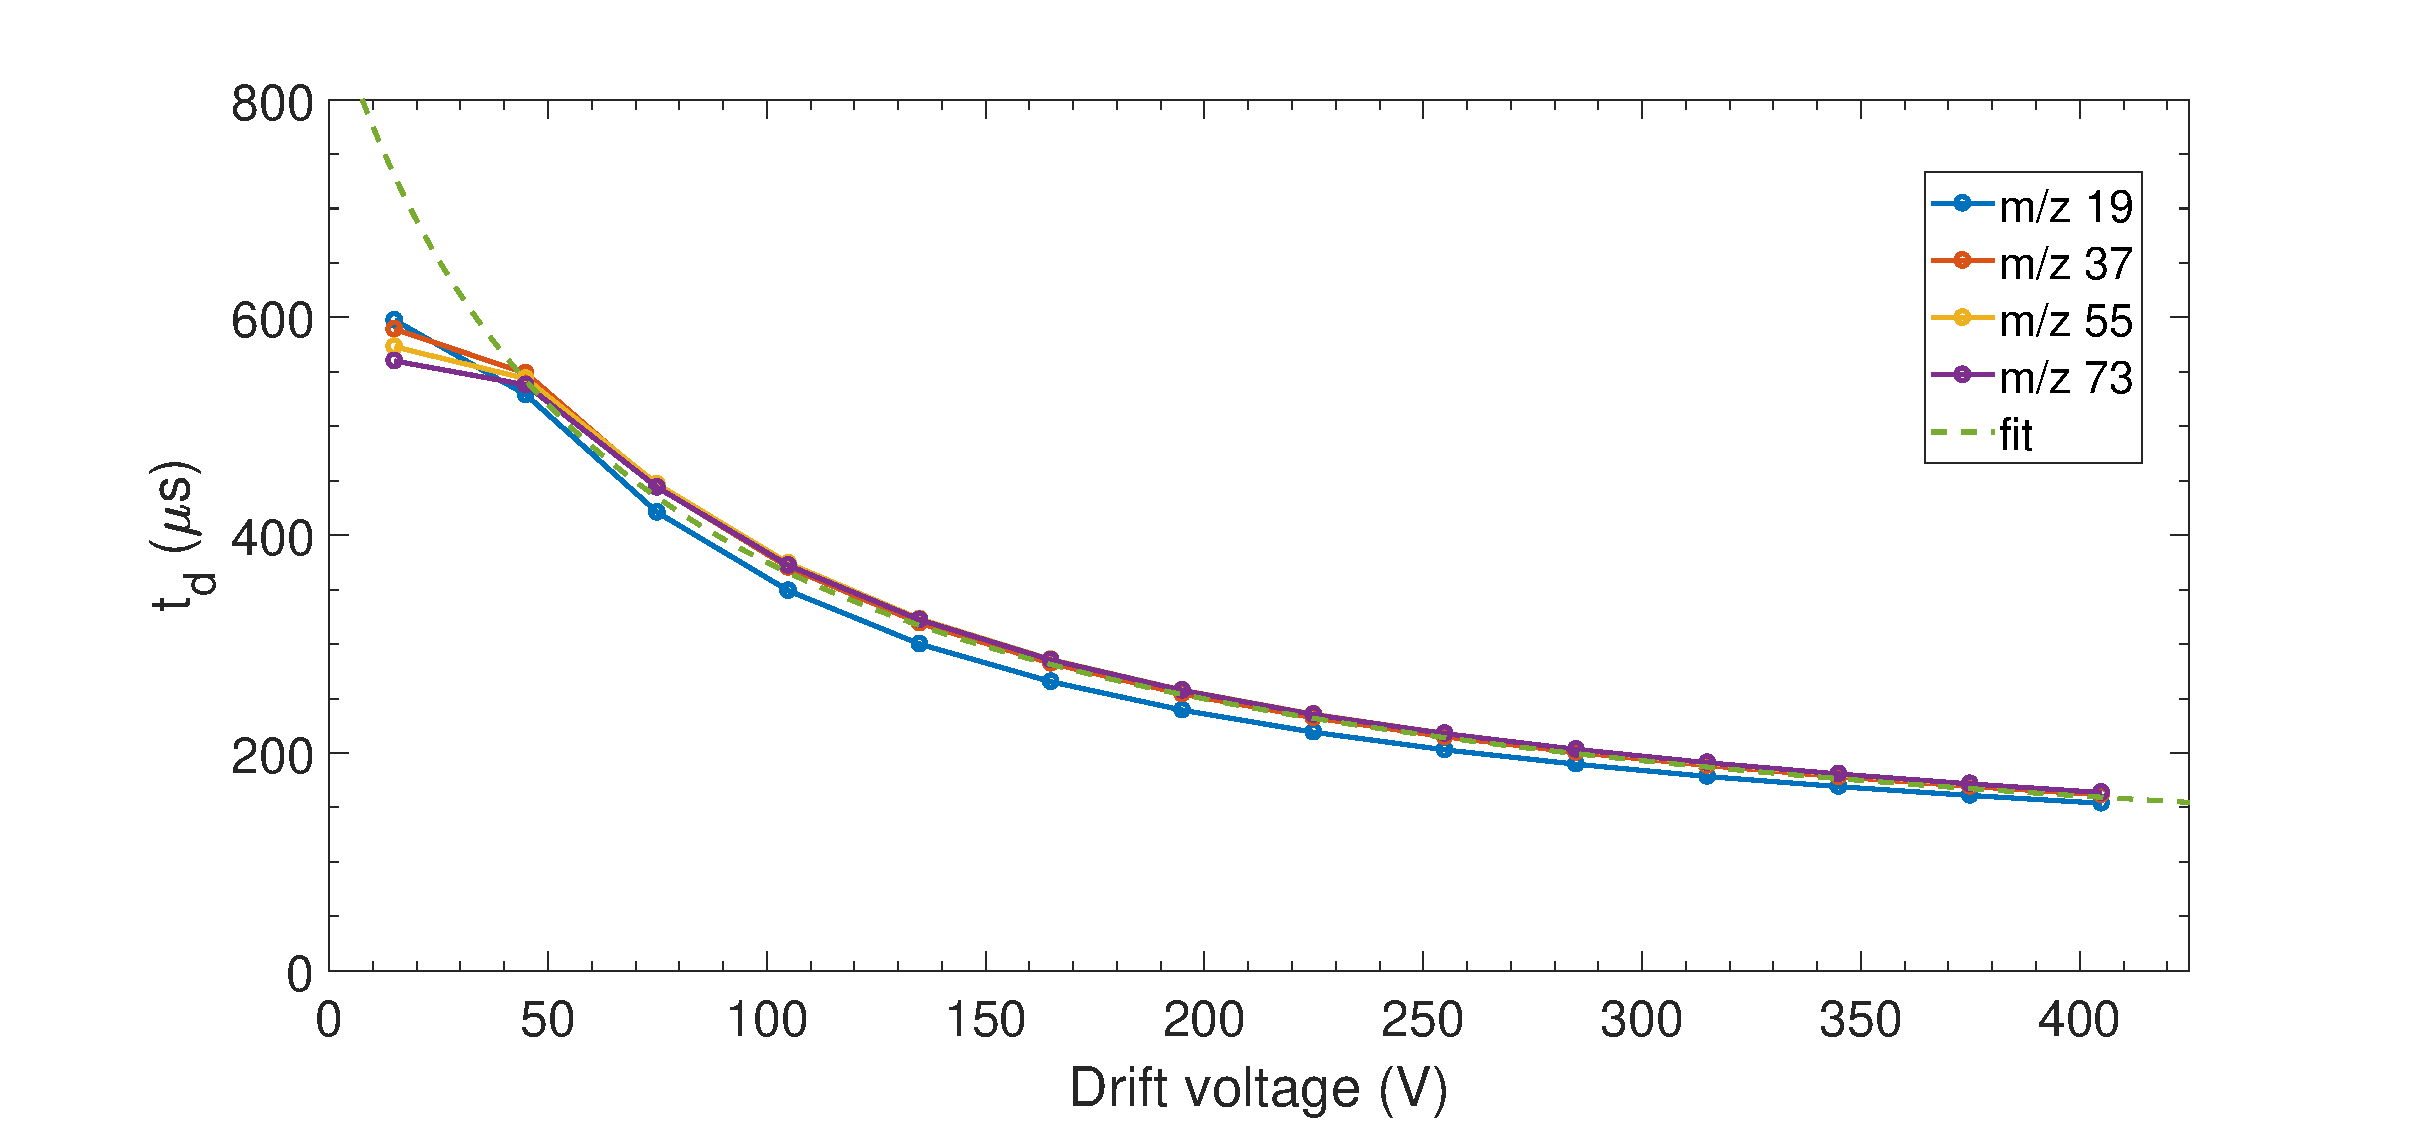
\includegraphics[width=0.9\linewidth]{pics/td_HS1.eps}\label{fig:td_DC}}

\bigskip
\sidesubfloat[]{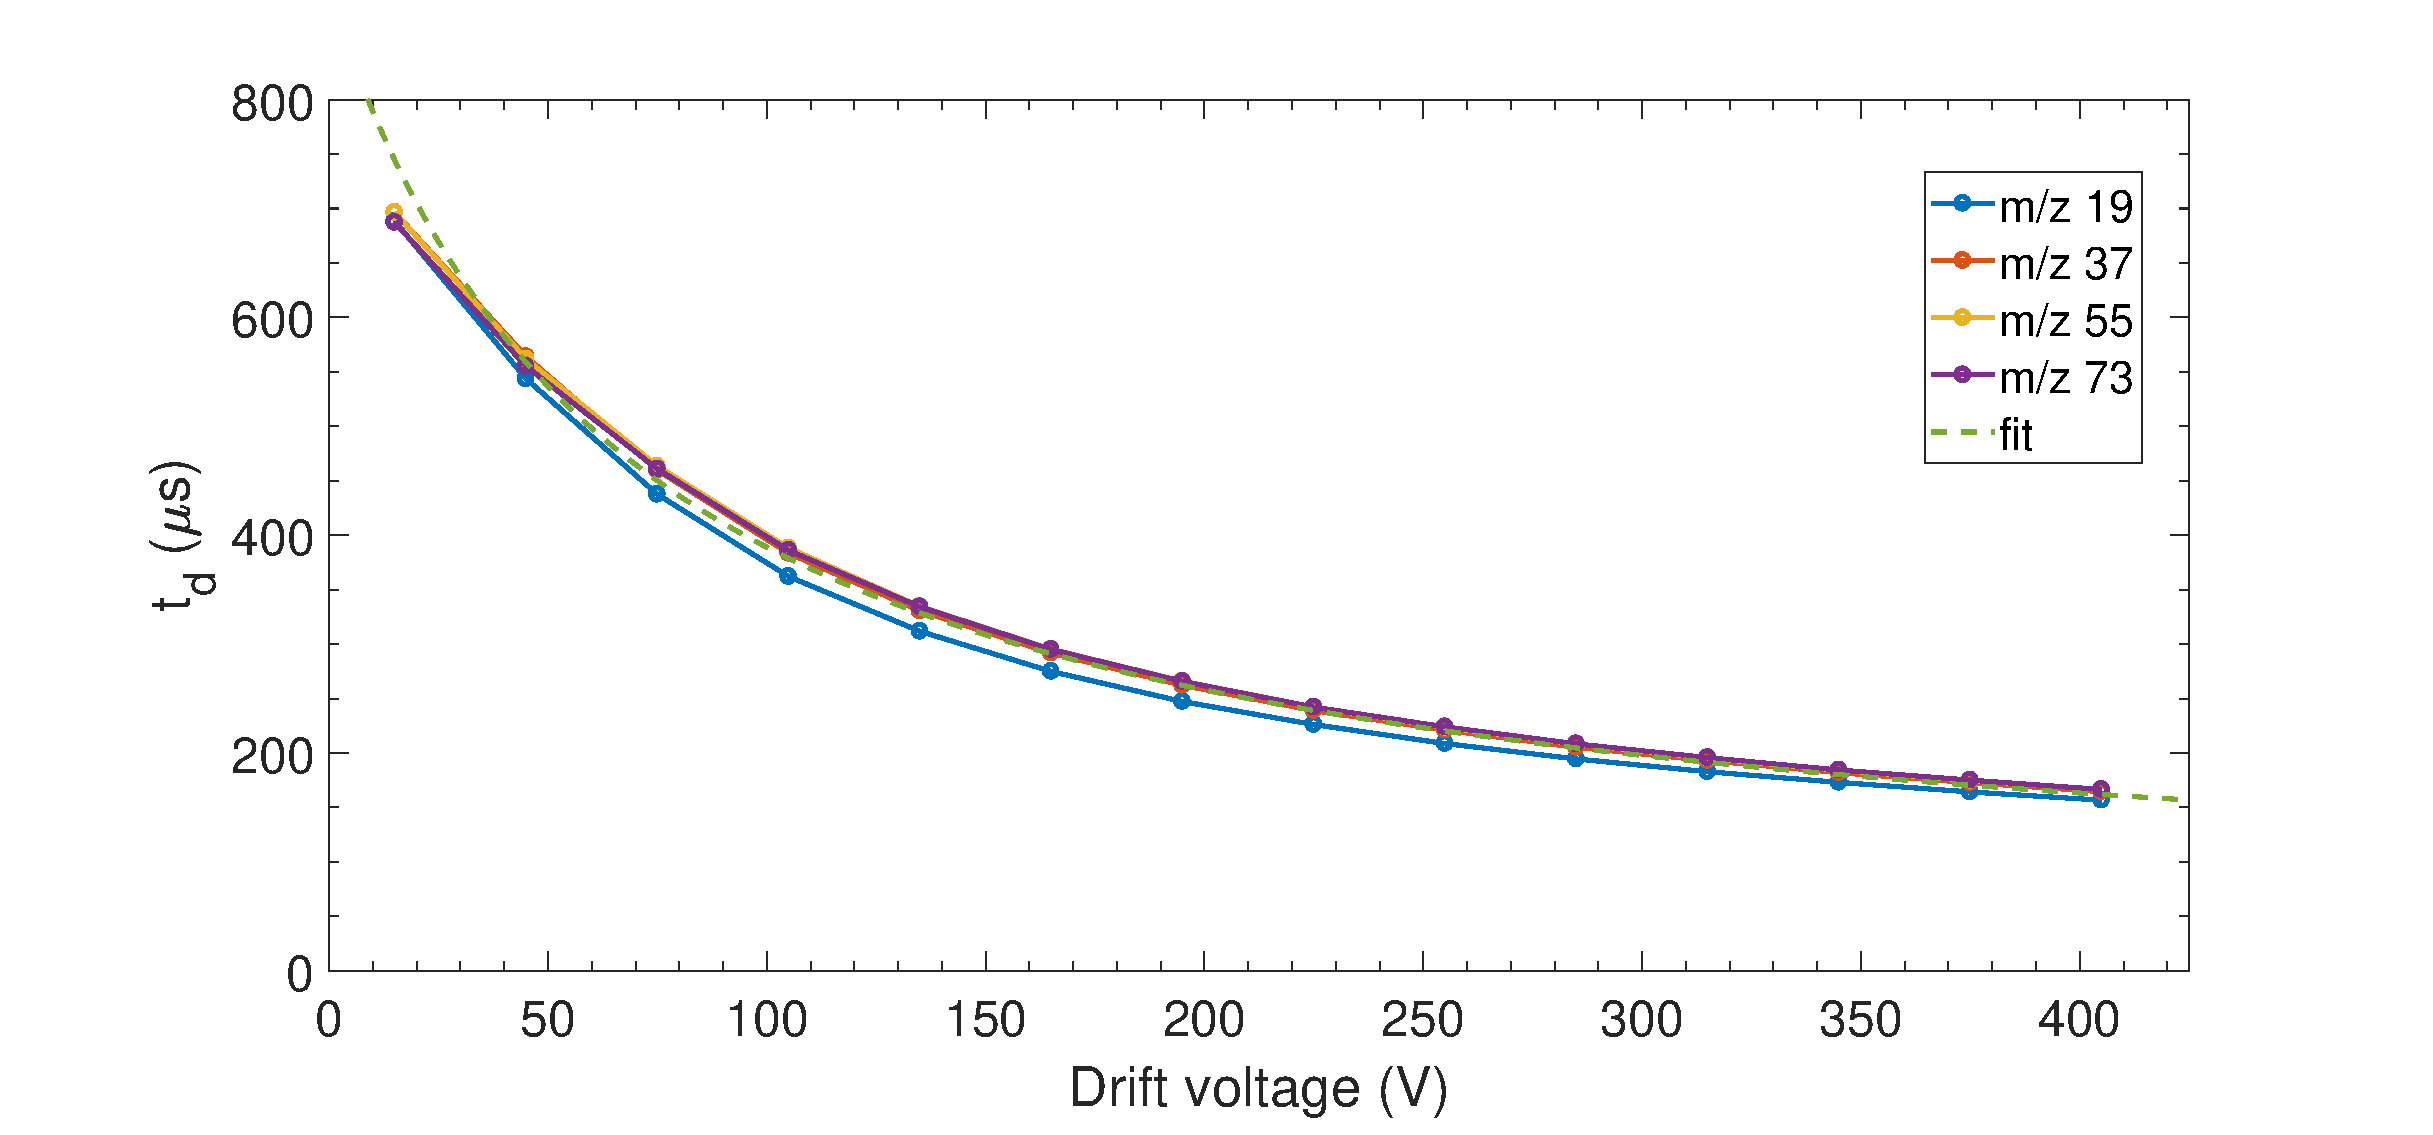
\includegraphics[width=0.9\linewidth]{pics/td_RF_HS1.eps}\label{fig:td_RF}}
\end{center}
\caption{Plot of the drift time, t$_d$, as a function of drift voltage for (a) DC mode and (b) RF mode. \textbf{THIS DATA IS OLD. THE NEW ONE NEEDS TO BE PLOTTED}}\label{fig:td}
\end{figure}







\subsection{Collisions in DC and RF mode}
I can also have a look at the number of collisions in each mode.
I can plot the kinetic energy vs the number of collisions for each mode


Compare DC and RF. Calculate the difference (in total and \%) of the collisions for both modes. This is shown in figure \ref{fig:col}.









\begin{figure}%[h]
\begin{center}
\sidesubfloat[]{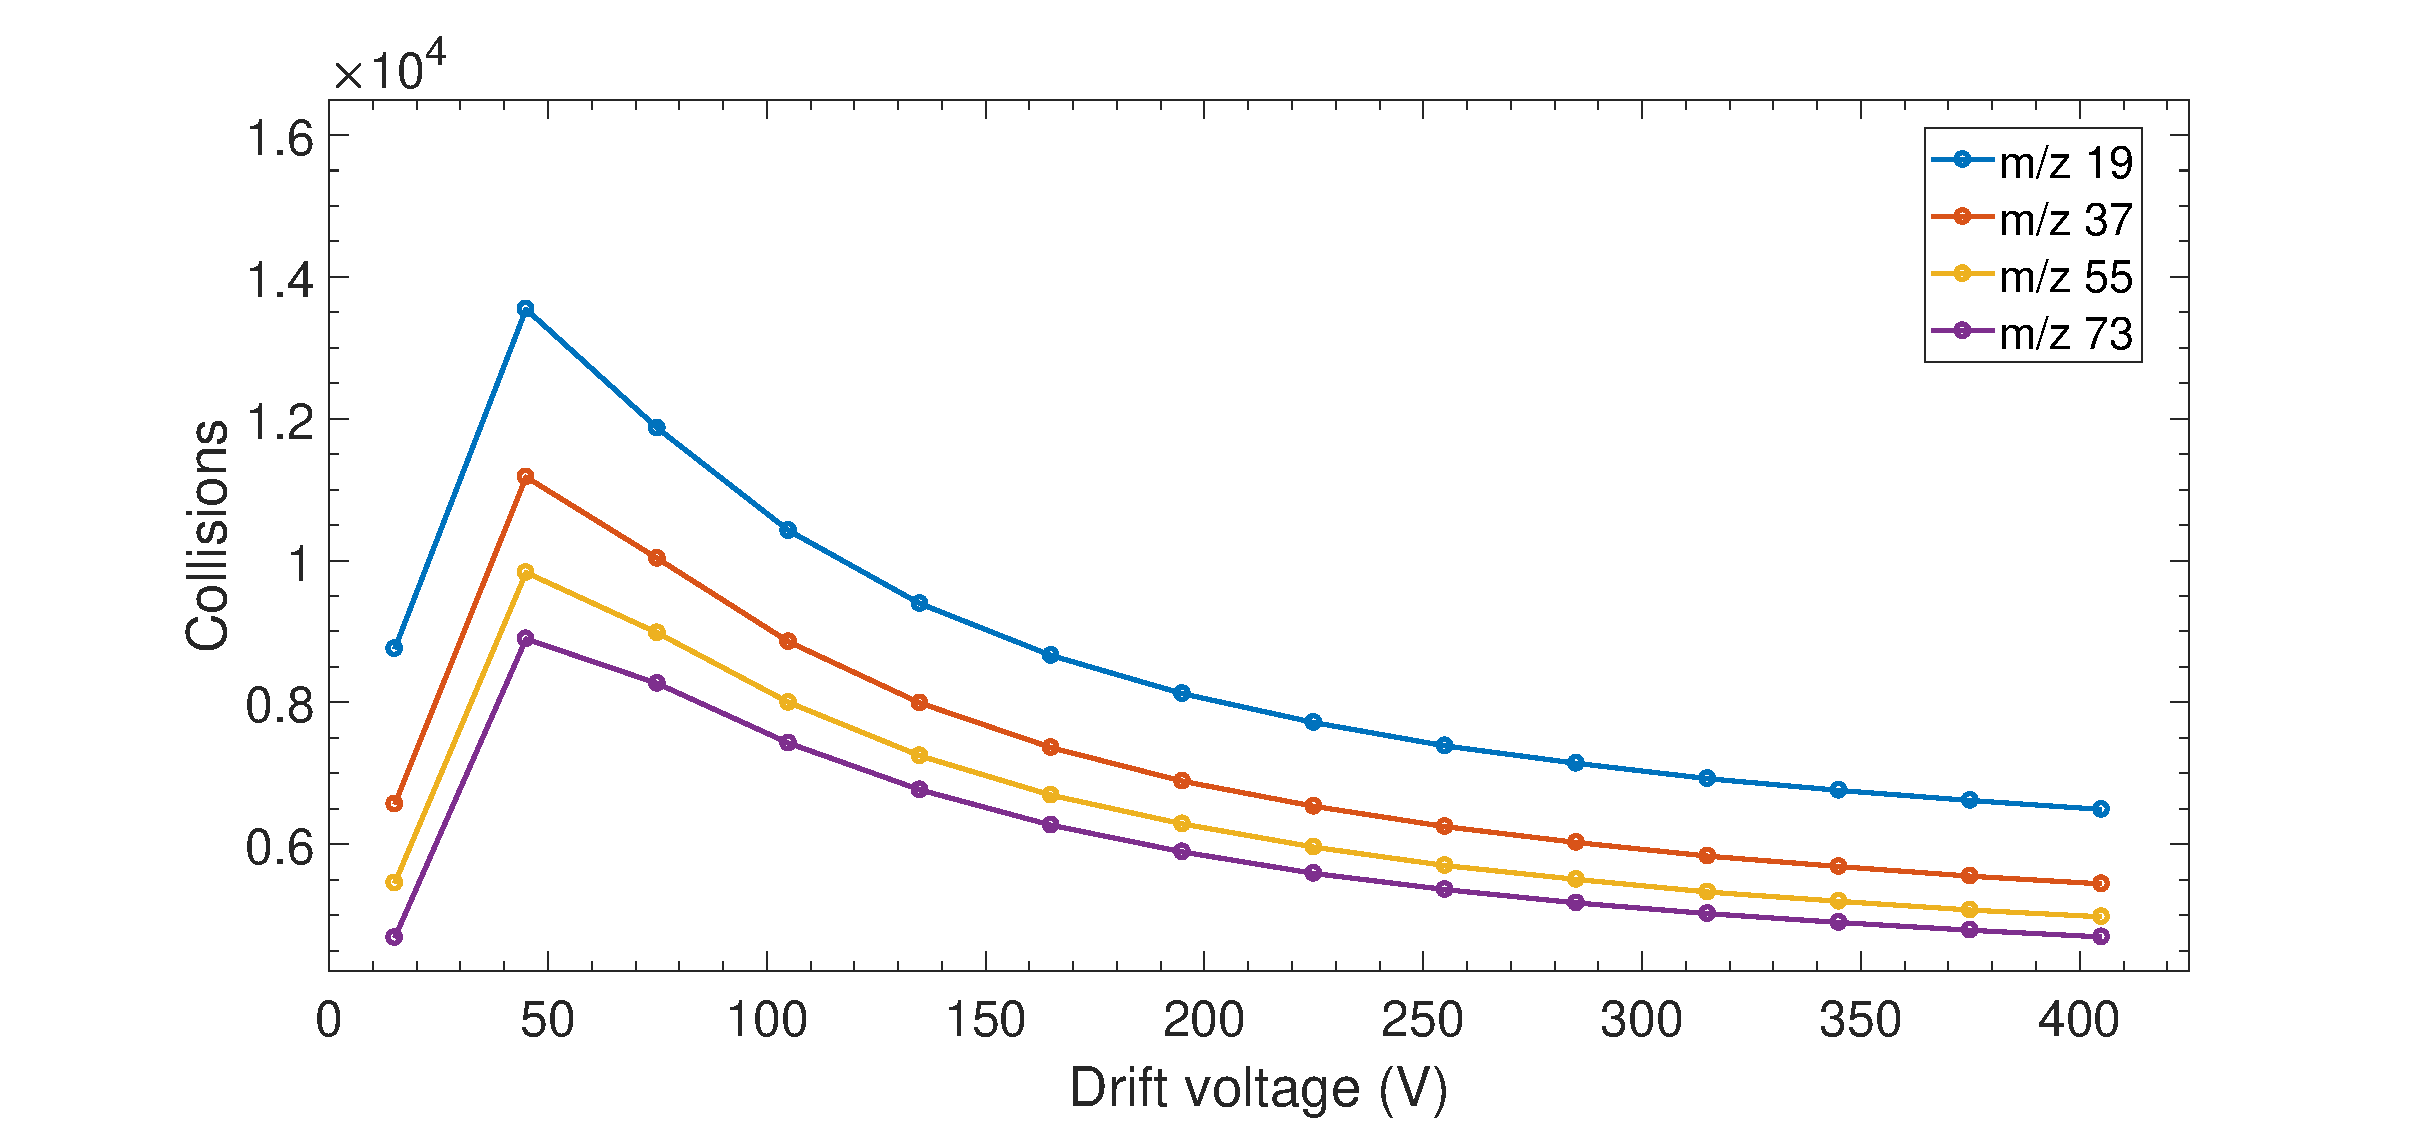
\includegraphics[width=0.9\linewidth]{pics/collisions_DC.eps}\label{fig:col_DC}}

\bigskip
\sidesubfloat[]{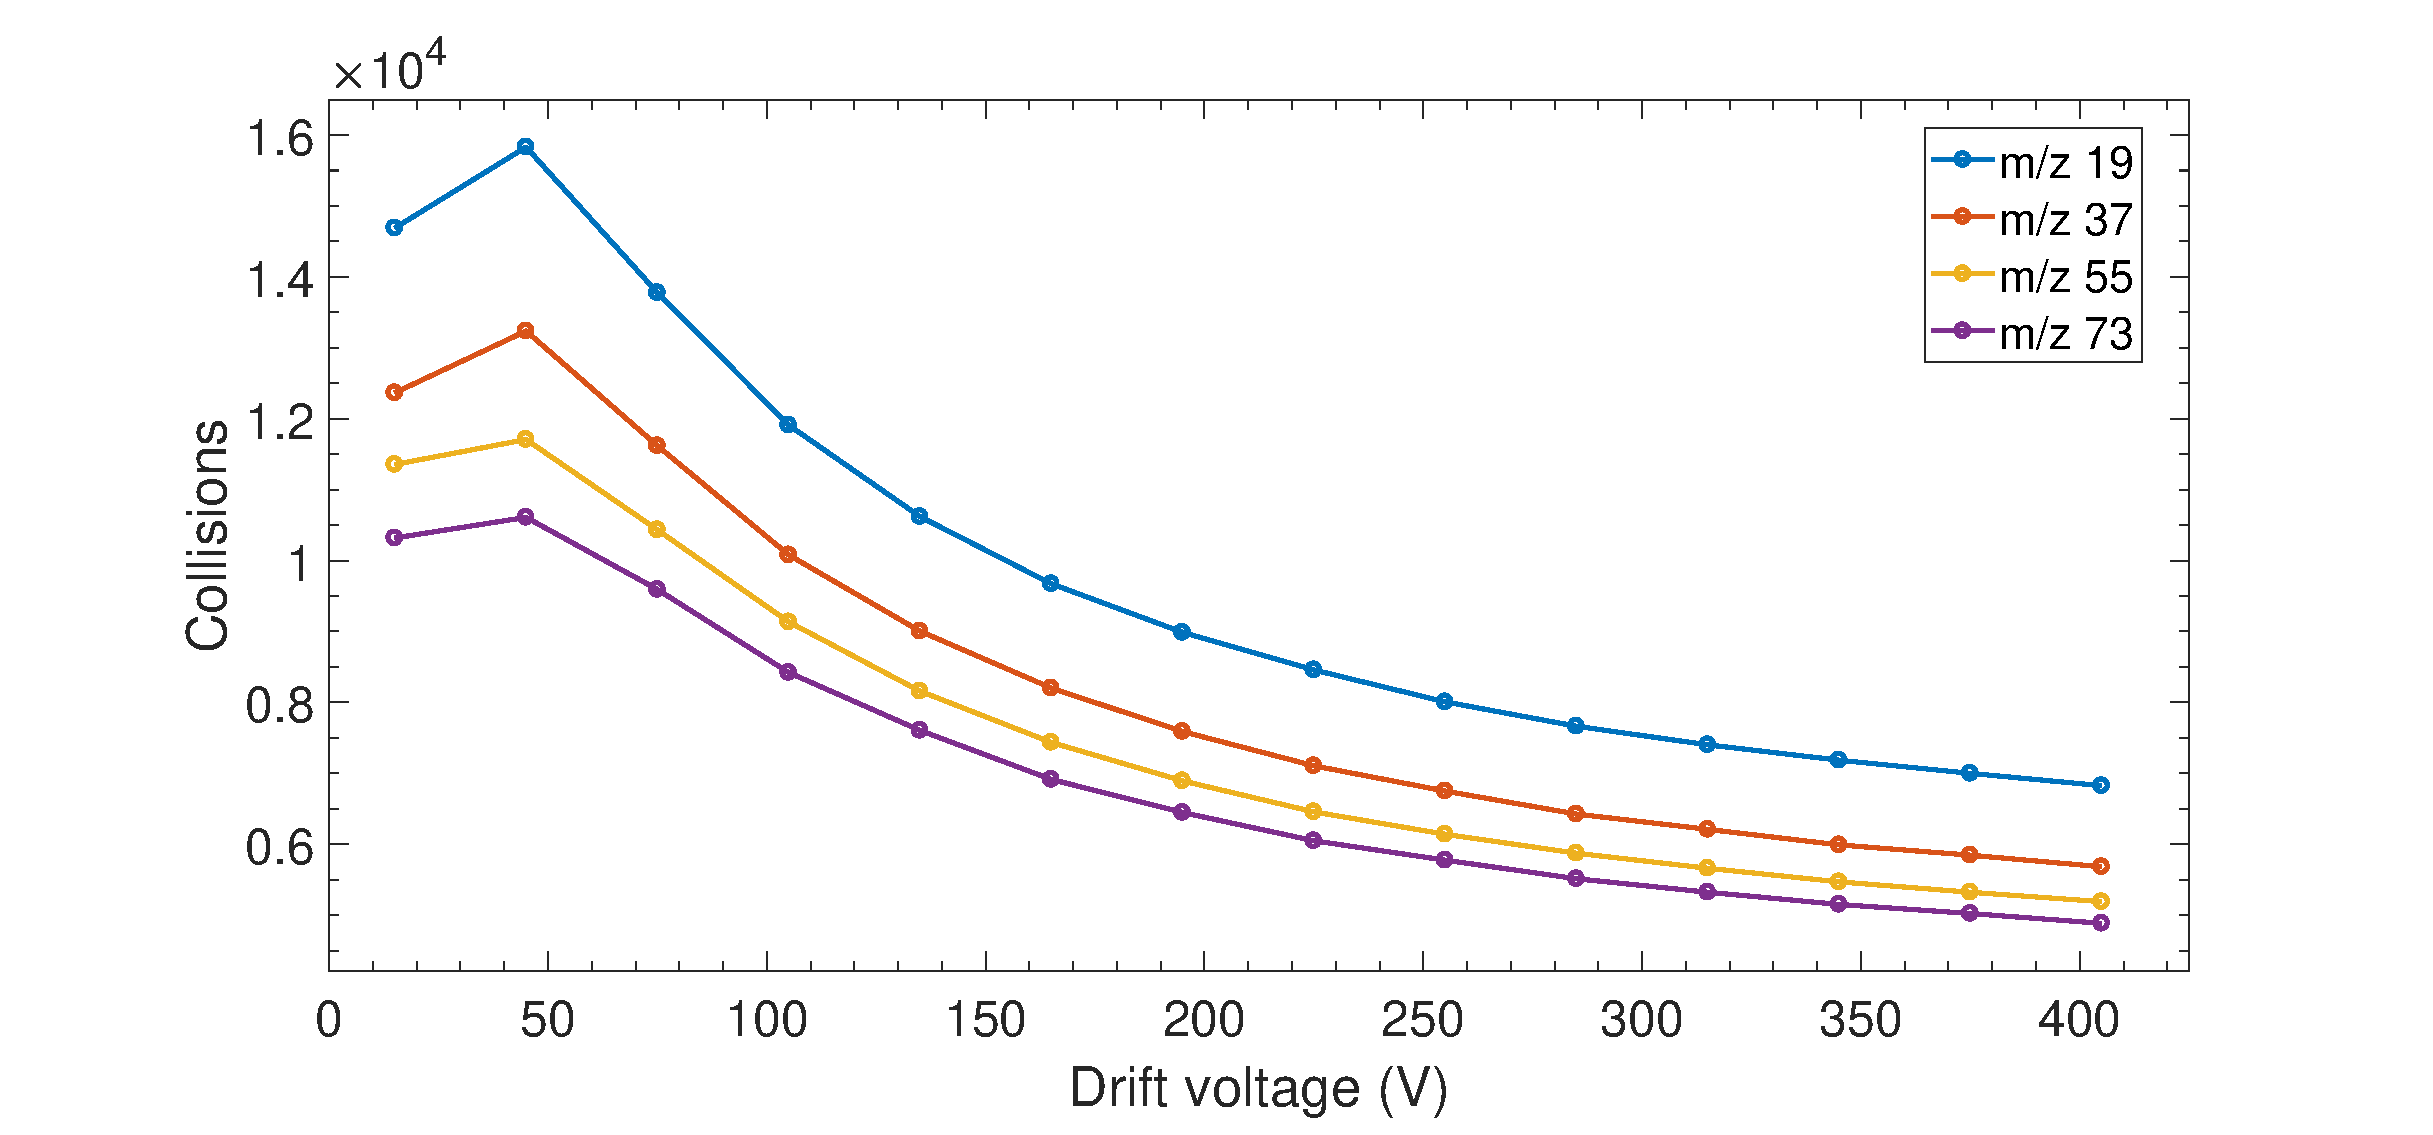
\includegraphics[width=0.9\linewidth]{pics/collisions_RF.eps}\label{fig:col_RF}}
\end{center}
\caption{Plot of the average number of collisions that every ion undergoes as a function of drift voltage for (a) DC mode and (b) RF mode }\label{fig:col}
\end{figure}













\subsection{Different configurations of the RF field}

The RF field voltage supplied to each of the plates, A$_{RF,n}$, can defined as:
\begin{equation}
A_{RF,n} = A_0\,sin\left(2 \pi f t + \phi_n    \right)
\label{eq:rf}
\end{equation}
\begin{equation}
\phi_n =  \frac{2 \pi n  }{n_p}
\label{eq:phase}
\end{equation}
where A$_0$ is 100 V (i.e. 200 V peak-to-peak), f is the linear frequency of the RF field (760 kHz), n indicates the n$^{th}$ plate, n$_p$ is a parameter to control the phase difference, t is the simulation time (in $\mu$s in SIMION, so the frequency must be converted to MHz), etc

Note that n$_p\,=\,2$ in the typical configuration of the RF field. This means that adjacent plates have opposite polarities, i.e. a phase difference of $\Delta\phi = \pi$, with $\Delta\phi = \phi_n - \phi_{n-1}$.

Note that for n$_p\,>\,2$ the RF field becomes a travelling wave, as opposed to a standing wave for n$_p\,=\,2$.

\begin{itemize}
\item Poner screenshots de ejemplos con n$_p$ 2,3,4 etc. de la superficie equipotencial y de la trajectoria de iones
\end{itemize}


\textbf{TO INCLUDE HERE: }
\begin{itemize}
\item simulations of transmission at low E/N (20 or 50V) for different values of np
\item Compare the different collisional models: the viscous model shouldn't take long to simulate. Pros and cons of each model: time consuming, precision, etc..
\item Do studies of average drift velocity as a function of E or E/N and as a function of the m/z of the ions (19,37,55,73) in DC and RF mode (can also be done for different values of n$_p$). With this, mobility can be calculated for each case (plot v$_d$ vs E)
\end{itemize}



\subsection{Calculation of the mobility of the reagent ions as a function of the E/N}
Run simulations and get v$_d$ as a function of E/N to get \acrshort{kk} from \ref{eq:vd}.
\begin{itemize}
\item Can I get the drift velocity along the whole reactor? Is it possible to get the acceleration?
\item Compare the ion mobility with the one in RF mode. Is it the same? Is it constant in any of the cases?
\item Can I extract (E/N)$_{effective}$ from this? (maybe I can explain this with a change of mobility or similar) (I could also just divide the equations)
\end{itemize}
 
Something else that I can do is to calculate the drift velocity in the first and second half of the stack in RF mode. 
\begin{itemize}
\item Does it change dramatically?
\item Compare the ion acceleration in the first and the second half of the stack to study RF acceleration.
\item Compare the drift velocity with the change in velocity with the RF mode (200V in 1/760kHz). Is it comparable?
\end{itemize}

\subsection{Flight path of the ions}
In RF mode the ions undergo more collisions. I can try to find a way to measure the travelled distance in RF and DC modes and compare them.




\subsection{Transmission as a function of the drift voltage}









To have a better idea of the transmission I considered that the number of ions that reach the exit plate are proportional to the ions transmitted through the exit aperture towards the differential pumping stage. The main reason for using the ions that reach the exit plate instead of the ones that go through the exit aperture is that it is more time efficient to use the former as the area of the exit plate is much bigger than that of the aperture.

The transmission, T, is calculated as a percentage following equation \ref{eq:sim_i}:
\begin{equation}
T = \frac{N_{exit}}{N_{f}} \times 100
\label{eq:sim_i}
\end{equation}
where N$_{exit}$ is the number of ions that hit exit plate from those flown, N$_f$. The averaged transmission is calculated following equation \ref{eq:sim_ia}:
\begin{equation}
T_{average} = 100 \times\frac{\sum_{i=1}^4 N_{exit,i}}{\sum_{i=1}^4 N_{f,i}} = \frac{1}{4}\sum_{i=1}^4T_i
\label{eq:sim_ia}
\end{equation}

Files:
\begin{itemize}
\item DC mode: \verb|16-35-24_09-January-2019_simulation-DC transmission-HS1 model| (1000 ions)
\item RF mode: \verb|14-46-57_27-April-2018_simulation|
\end{itemize}


Figure \ref{fig:sim} shows the transmission study for DC and RF modes for hydronium and the first three water clusters (N=20000, grouped, factor = 10$^6$)

Transmission is mass-dependent in RF mode while it is not in DC mode. 

Transmission increases with the drift voltage in all cases.

This low-mass cut-off of RF funnels has been reported in the literature already \cite{Chung123}



\begin{figure}%[h]
\begin{center}
\sidesubfloat[]{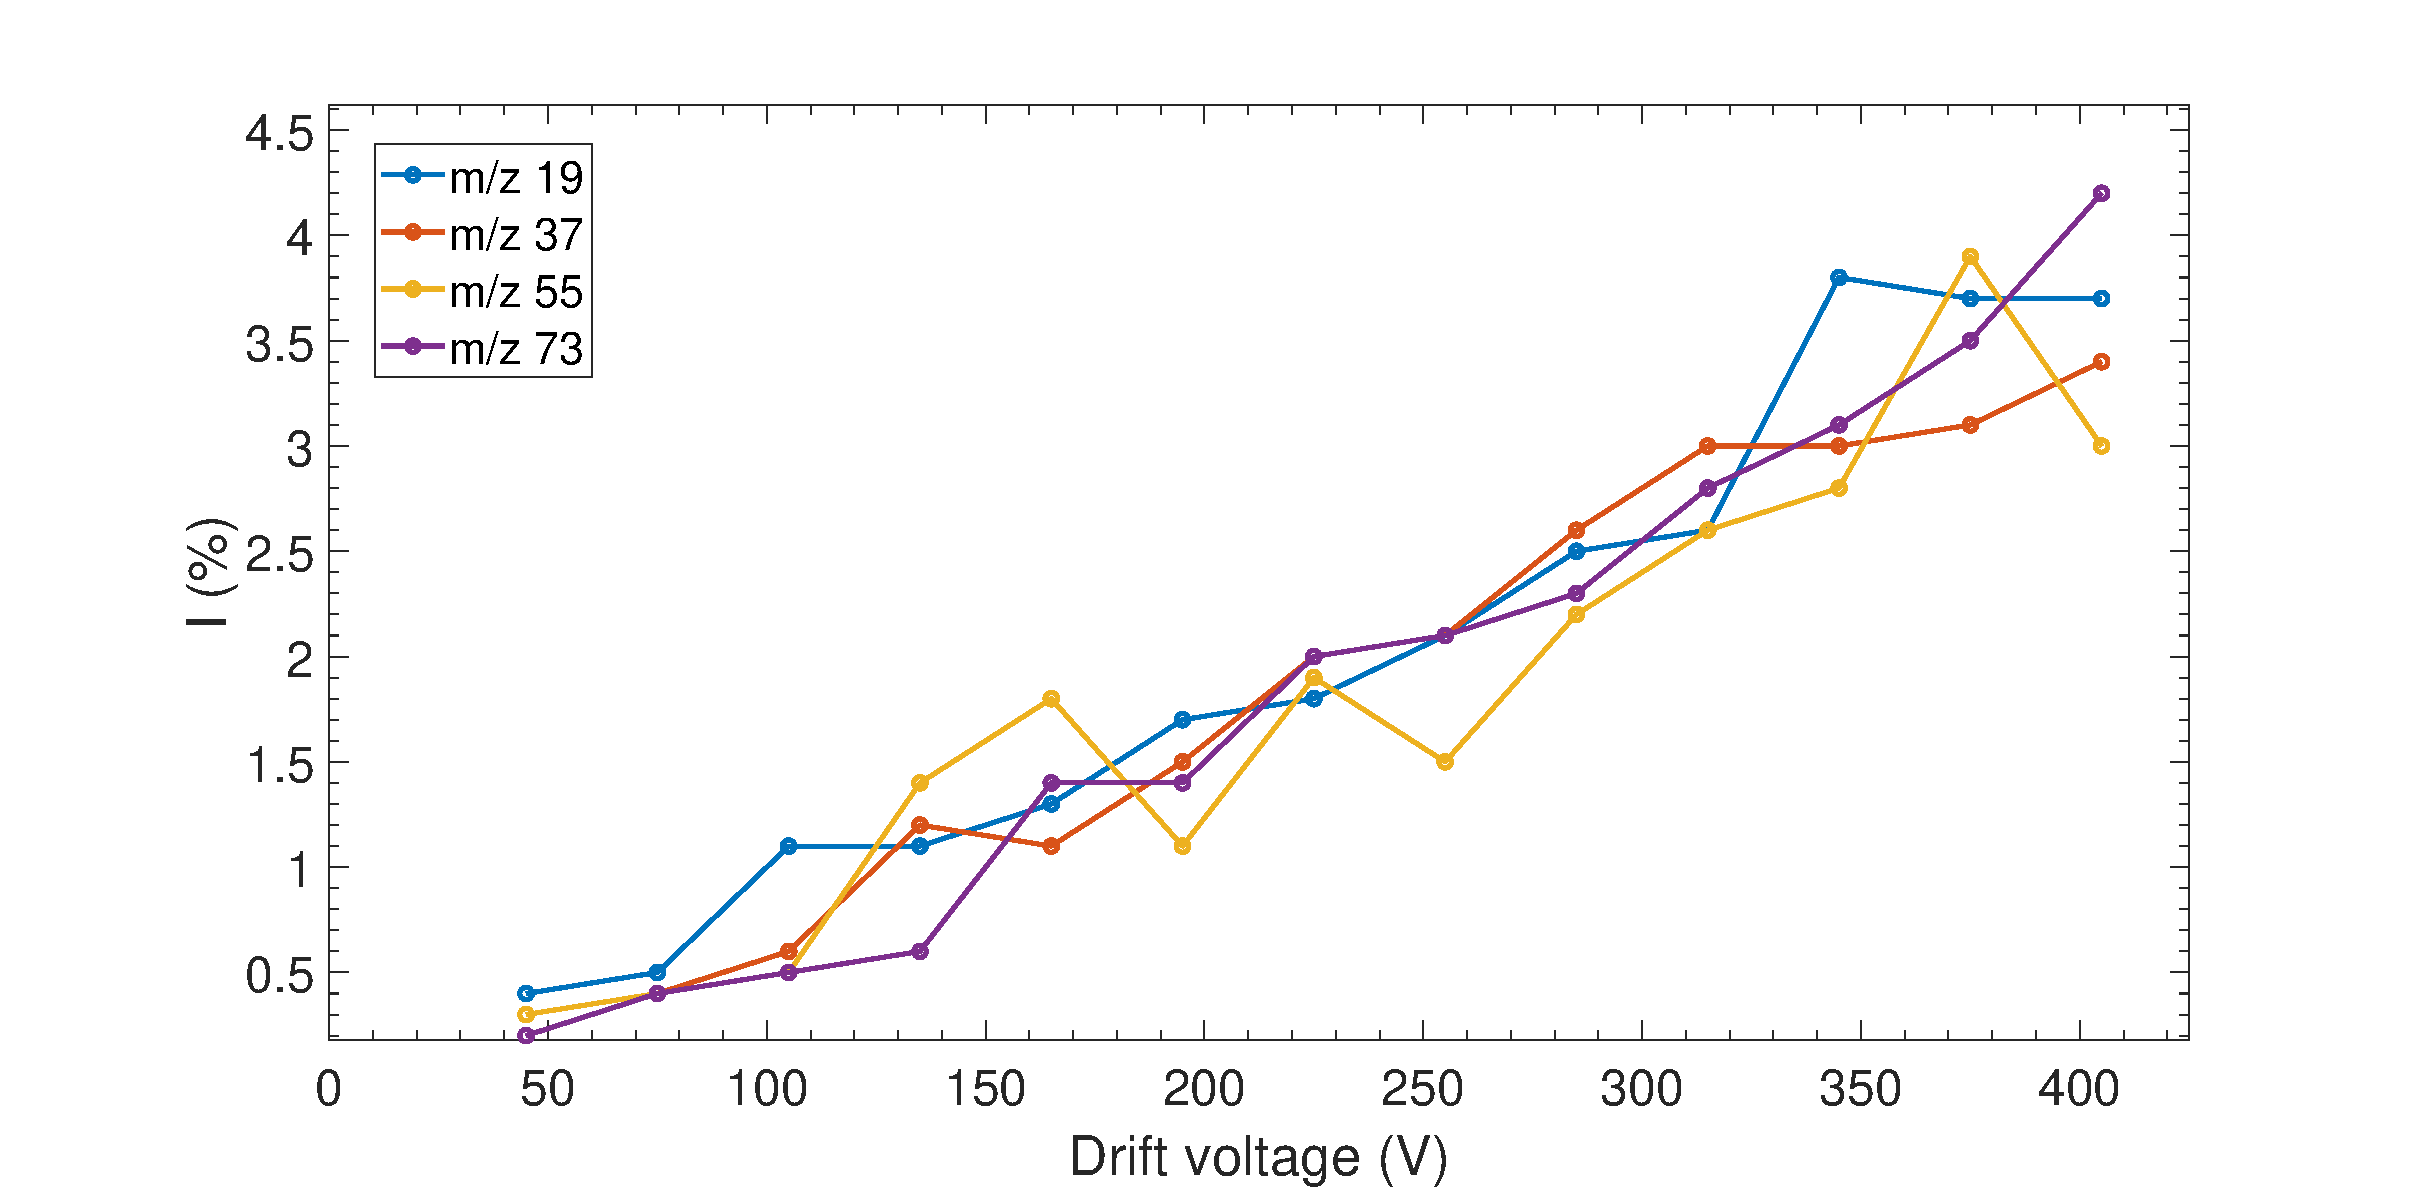
\includegraphics[width=0.75\linewidth]{pics/DC_HS1_1000ions.eps}\label{fig:sim_DC}}

\sidesubfloat[]{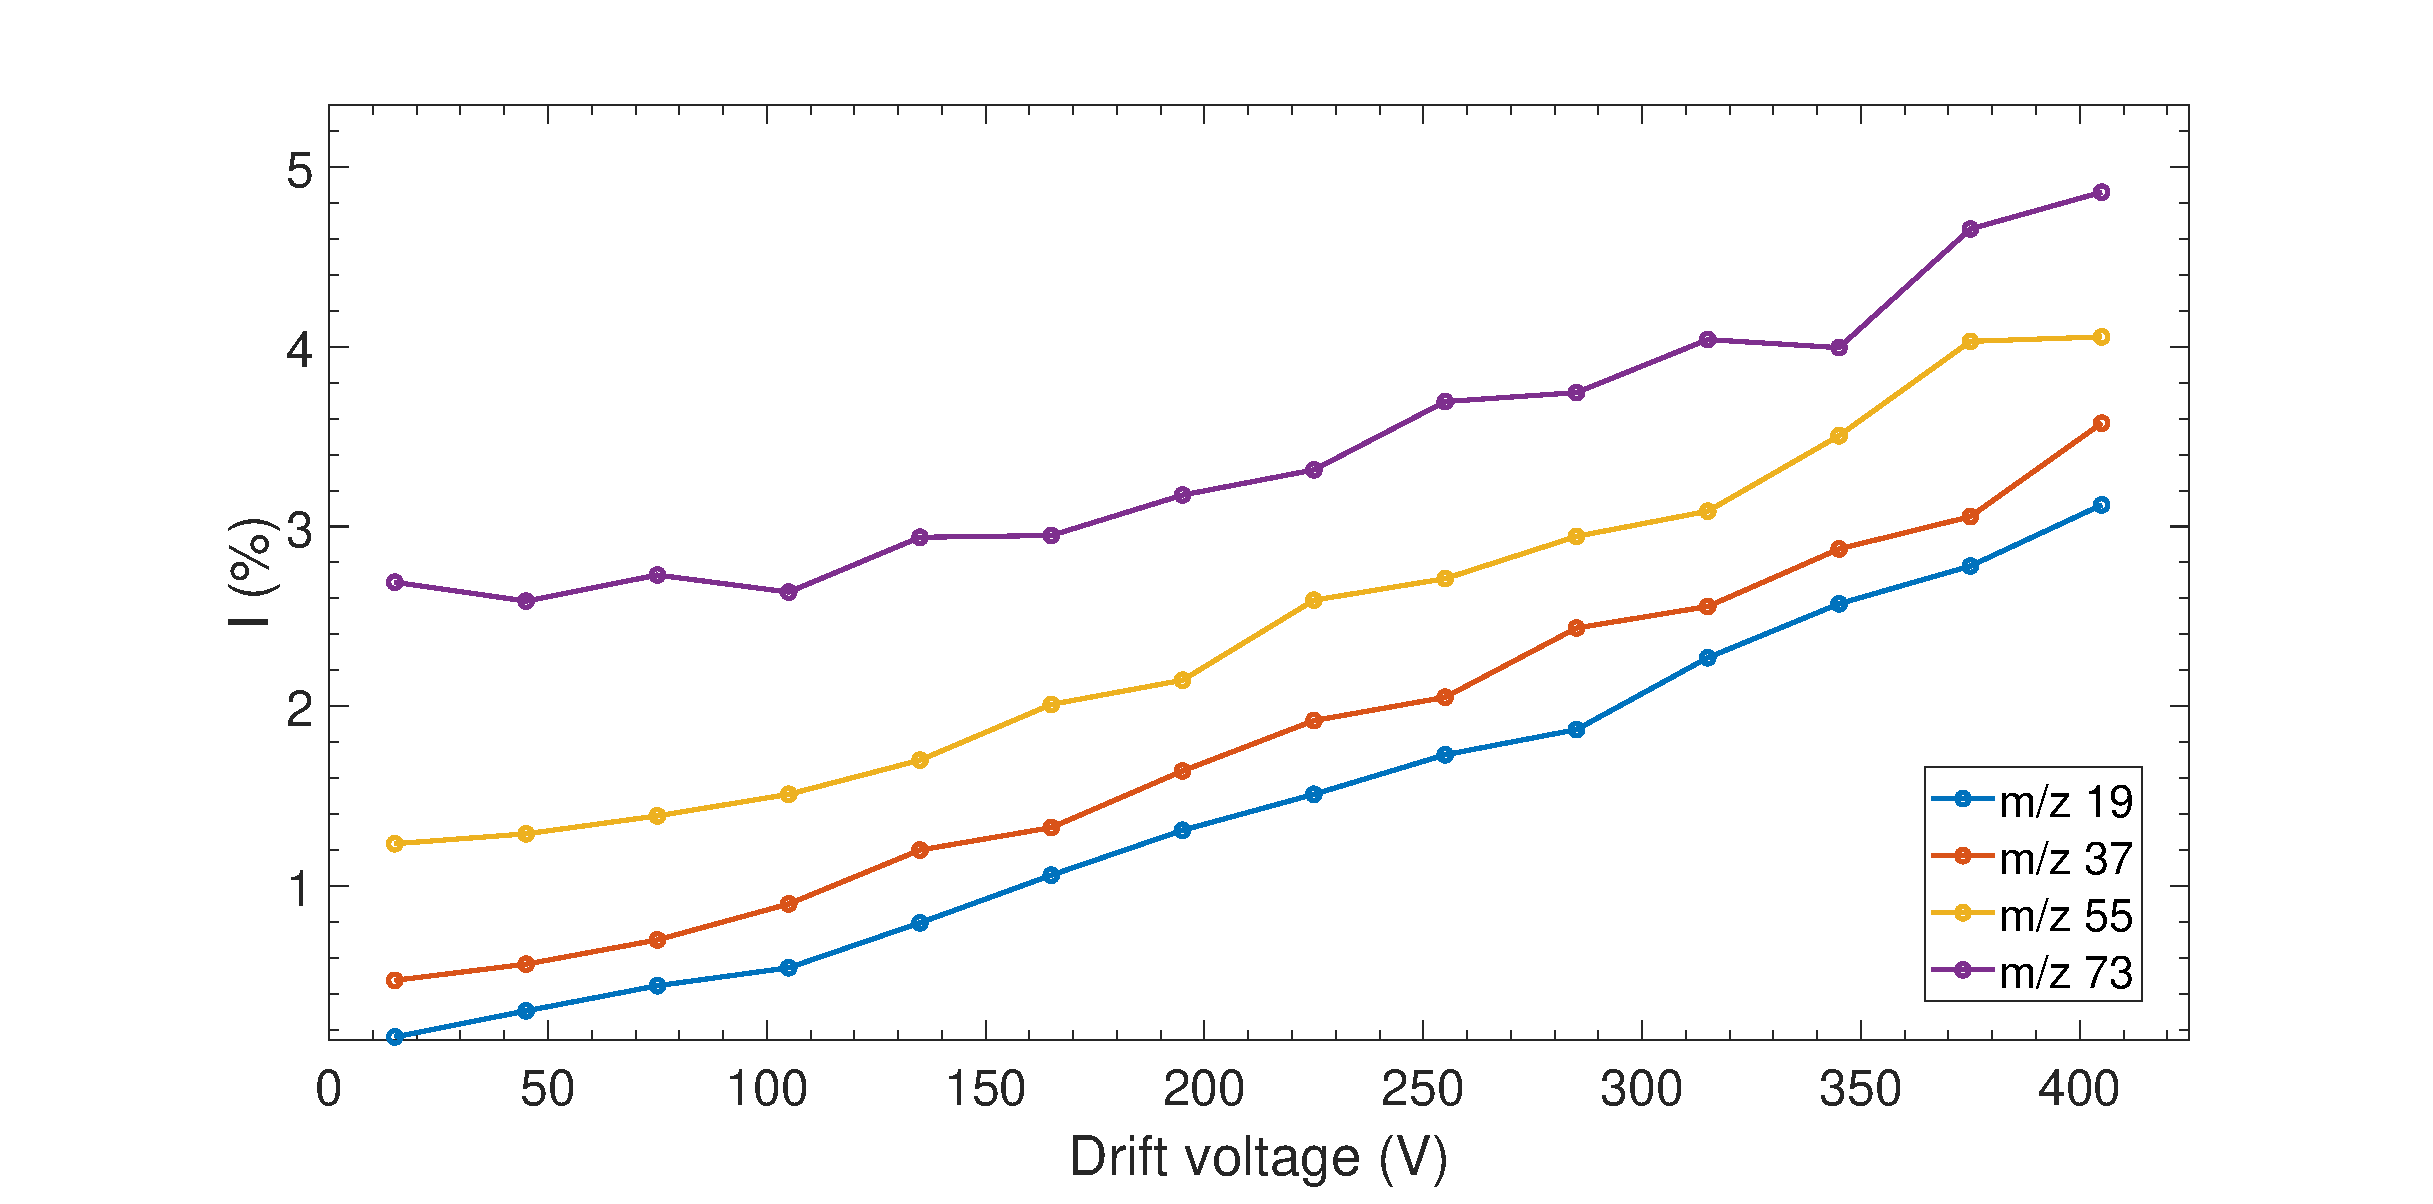
\includegraphics[width=0.75\linewidth]{pics/RF_HS1_20000ions.eps}\label{fig:sim_RF}}

\sidesubfloat[]{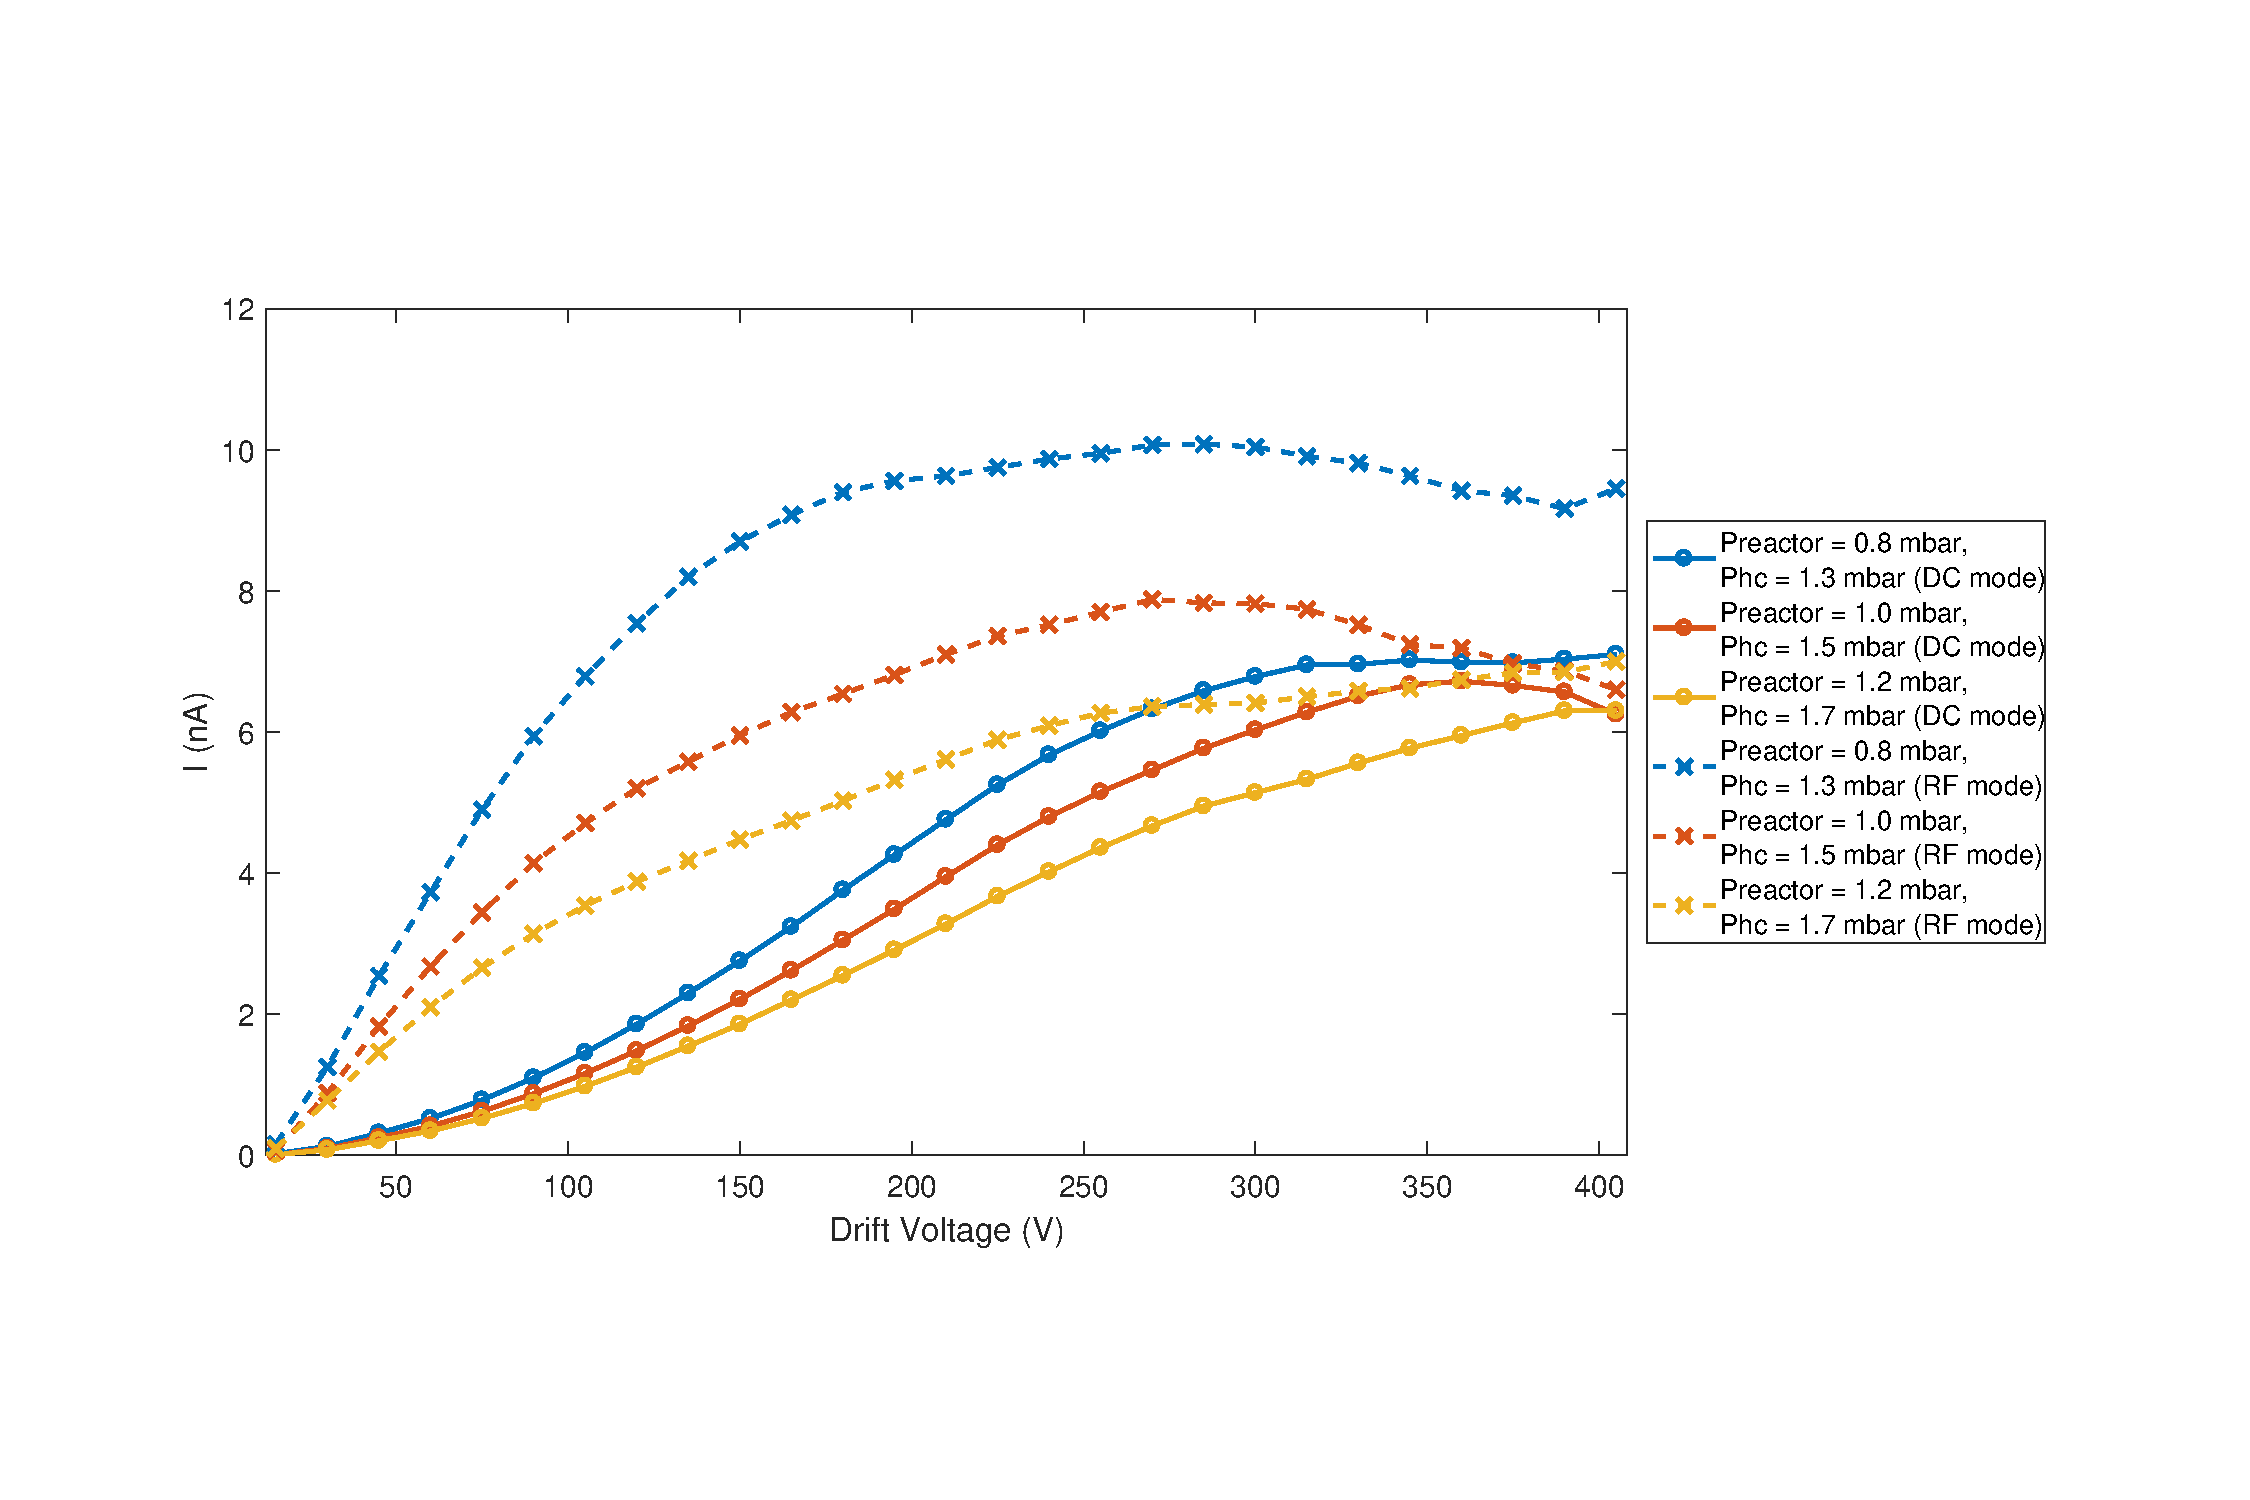
\includegraphics[width=0.75\linewidth]{pics/transmission_p.pdf}\label{fig:current_plot}}
\end{center}
\caption[Percentage of ions that reach exit plate as a function of the drift voltage for hydronium and the first water cluster ions]{Percentage of ions that reach exit plate as a function of the drift voltage for hydronium and the first water cluster ions. HS1 model, 1000 ions for DC mode and 20000 ions for RF mode.}\label{fig:sim}
\end{figure}








\section{Current density}
Can this be calculated in SIMION?

\newpage
\section{Comparison with SDS model}
See SDS User Program documentation

The statistical diffusion simulation model (SDS) is more time efficient than the hard sphere model HS1 as it employs collision statistics rather than simulate each individual collision \cite{APPELHANS20051}.




The SDS model needs the diameter (hard sphere) and/or reduced mobility of the ions before starting the simulation. %As we are interested mainly in (H$_2$O)$_n$H$_3$O$^+$, we need their reduced mobilities. 
For (H$_2$O)$_n$H$_3$O$^+$ (n=0, 1, 2) they can be found in \cite{Dotan}. SDS takes K$_0$ as constants, i.e. no E/N dependence, so an average over the E/N range provided in the literature will be used as approximation. This yields  2.9$\times$10$^{-4}$, 2.4$\times$10$^{-4}$ and 2.2$\times$10$^{-4}$ m$^2$ V$^{-1}$ s$^{-1}$ for H$_3$O$^+$, (H$_2$O)H$_3$O$^+$ and (H$_2$O)$_2$H$_3$O$^+$, respectively. However, if K$_0$ is not provided, it is automatically calculated. If the ion's diameter is not provided either, it is calculated from the empirical equation \ref{eq:sds1}, which assumes that the density is constant across the whole volume:
\begin{equation}
\label{eq:sds1}
d_{ion} = 0.120415405 \times \sqrt[3]{mass_{ion}}
\end{equation}
where d$_{ion}$ is in nm and mass$_{ion}$ in amu. Once d$_{ion}$ is known, K$_0$ is calculated from equation \ref{eq:sds2}:
\begin{equation}
\label{eq:sds2}
K_0 = 10^{-5} \times 10^A
\end{equation}
\begin{equation}
A = 4.9137 - 1.4491 (\log_{10} (d_{ion}) - 0.2772\log_{10} (d_{ion}))^2 + 0.0717 (\log_{10} (d_{ion}))^3
\end{equation}
where K$_{0}$ is in m$^2$ V$^{-1}$ s$^{-1}$. This approximation can be used for (H$_2$O)$_3$H$_3$O$^+$, whose reduced mobility in N$_2$ is not found in the literature, and it gives an estimated value of 2.11$\times$10$^{-4}$ m$^2$ V$^{-1}$ s$^{-1}$, which seems coherent with that for the other ions. 










\textbf{To include here:}
\begin{itemize}
\item Show with SDS diffusion = 0 that for RF parameter = 2 there are potential wells where small ions (m/z 19) can get trapped, while for RF parameter = 3 this doesn't happen. Explain that SDS diffusion is set to 0 to see the effect more clearly but it also happens with SDS diffusion = 1, or at least the residence time is much higher, until the diffusion takes the ion out of the stable trajectory.
\end{itemize}




\begin{figure}%[h]
\begin{center}
\sidesubfloat[]{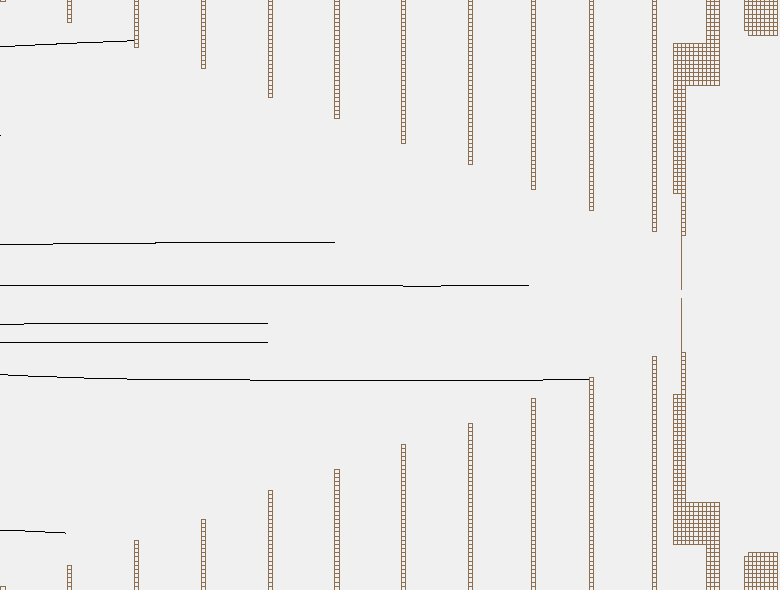
\includegraphics[width=0.35\linewidth]{pics/t01.png}}
\sidesubfloat[]{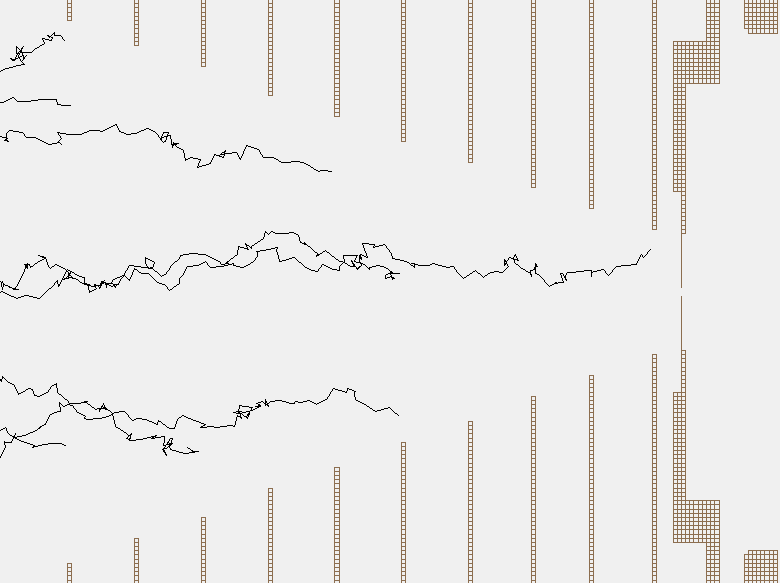
\includegraphics[width=0.35\linewidth]{pics/t11.png}}\\ \bigskip
\sidesubfloat[]{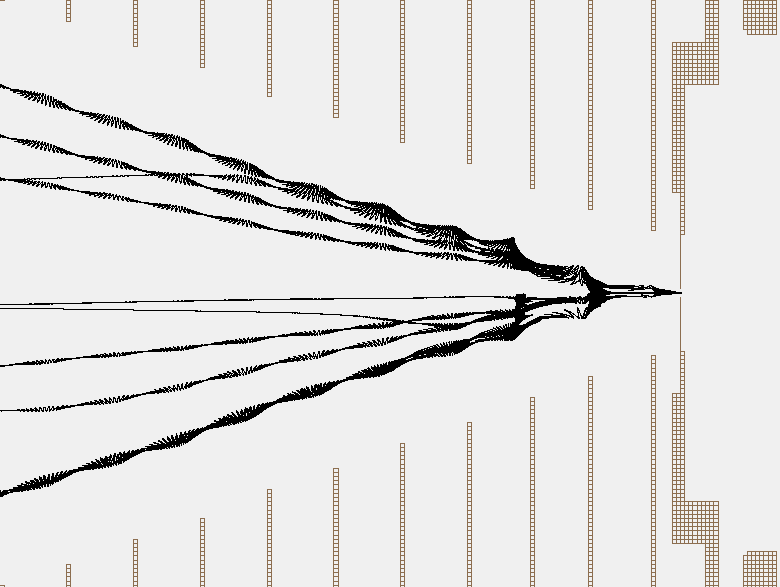
\includegraphics[width=0.35\linewidth]{pics/t02.png}}
\sidesubfloat[]{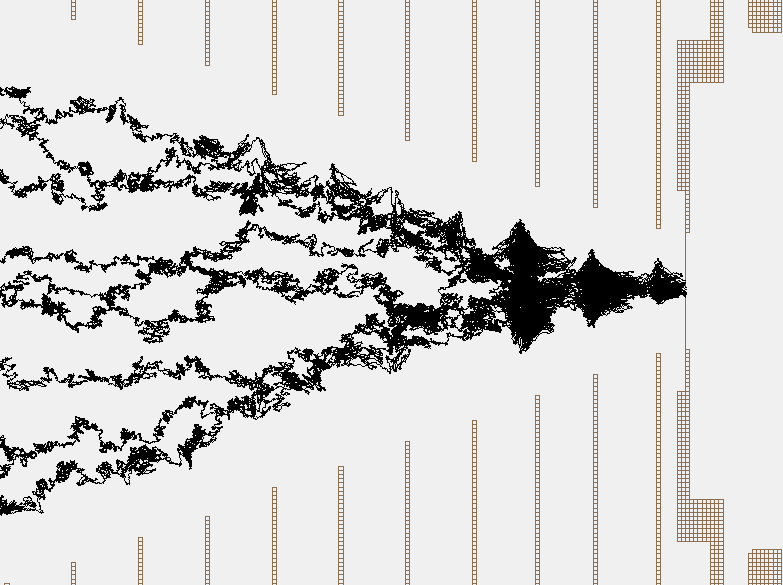
\includegraphics[width=0.35\linewidth]{pics/t12.png}}\\ \bigskip
\sidesubfloat[]{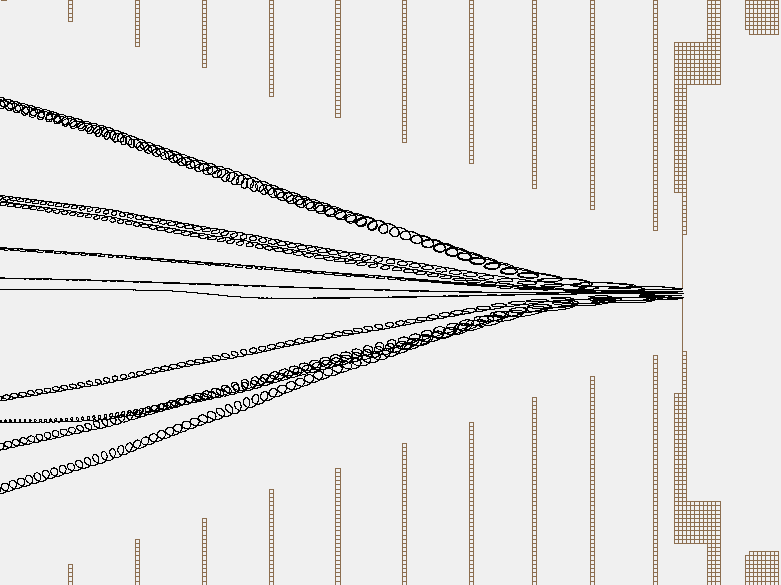
\includegraphics[width=0.35\linewidth]{pics/t03.png}}
\sidesubfloat[]{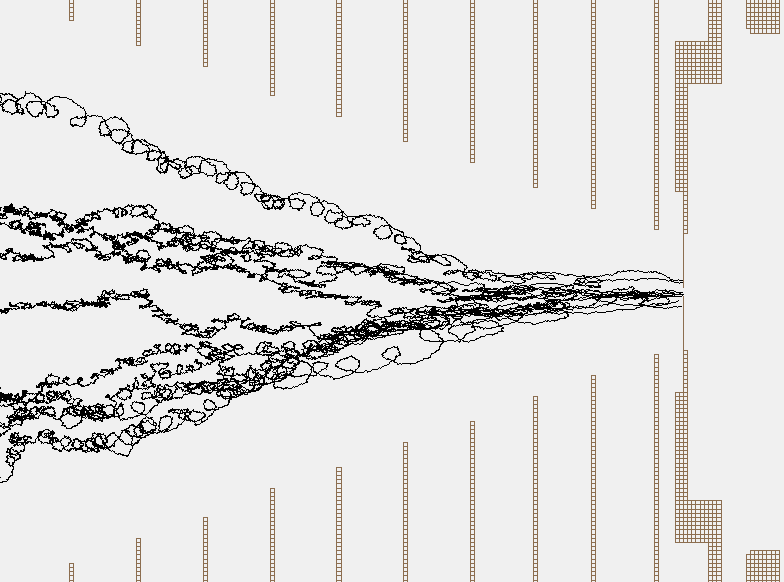
\includegraphics[width=0.35\linewidth]{pics/t13.png}}\\ \bigskip
\sidesubfloat[]{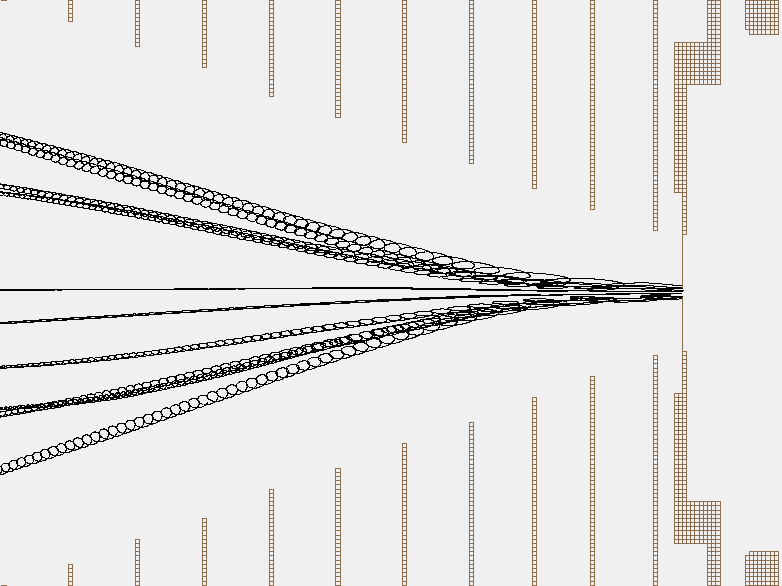
\includegraphics[width=0.35\linewidth]{pics/t04.png}}
\sidesubfloat[]{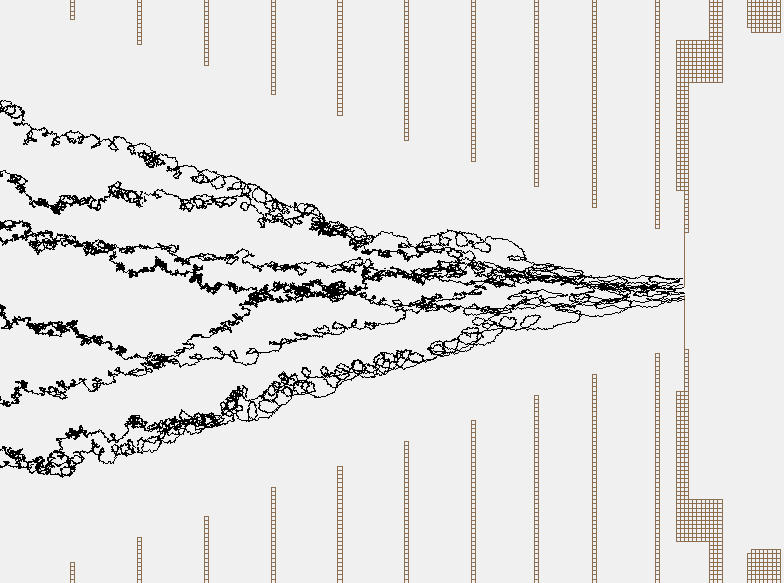
\includegraphics[width=0.35\linewidth]{pics/t14.png}}\\ \bigskip
\end{center}
\caption[Comparison of the trajectories of 10 ions of m/z 19 in different conditions]{Comparison of the trajectories of 10 ions of m/z 19 in different conditions. DC mode (a,b), RF mode: $\Delta \phi$ = 180$^{\circ}$ (c,d), $\Delta \phi$ = 120$^{\circ}$ (e,f) and $\Delta \phi$ = 90$^{\circ}$ (g,h). Note that for the images in the left column there was no diffusion enabled while for the right one the diffusion was enabled.
}\label{fig:traj}
\end{figure}


\subsection{Drift time}
Files:
\begin{itemize}
\item DC mode: \verb|David Olivenza sds model\excel\SDS_drift time_DC|
\item RF mode: \verb|David Olivenza sds model\excel\SDS_drift time_RF|
\end{itemize}

Assuming DC mode (no RF field) and motion in 1D, the forces on the ion:
\begin{equation}
m\frac{d^2x}{dt^2} = eE - k_1\frac{dx}{dt} + k_2 v_{buffer}
\end{equation}
The first term corresponds to the electrostatic force, the second one is the dampening effect due to the collisions with the buffer gas and the third one is the dragging effect due to the non-zero velocity of the buffer gas.
For a steady velocity, i.e. $\frac{d^2x}{dt^2} = 0$, yields
\begin{equation}
\frac{dx}{dt} = \frac{1}{k_1} \left( eE + k_2 v_{buffer} \right)
\end{equation}
So the drift time, i.e. $t_d = L/\frac{dx}{dt}$, is:
\begin{equation}
t_d = \frac{k_1 L}{eE +k_2 v_{buffer}} = \frac{k_1 L}{eV_d/L + k_2 v_{buffer}} = \frac{k_1 L^2/e}{V_d + k_2 L v_{buffer}/e}
\end{equation}
which can be written as:
\begin{equation}
t_d = \frac{C_1}{V_d + C_2}
\label{eq:sds_t}
\end{equation}


Note that:
\begin{equation}
t_d(V_d\rightarrow0) \rightarrow \frac{C_1}{C_2} \approx  t_{buffer}
\end{equation}
This drift time is purely coming from convection. If no electric field was applied to the drift tube, the drift time would be:
\begin{equation}
t_{buffer} = \frac{L}{v_{buffer}} = \frac{9.36\,cm}{100\,m/s} = 936\, \mu s
\end{equation}






\begin{figure}%[h]
\begin{center}
\sidesubfloat[]{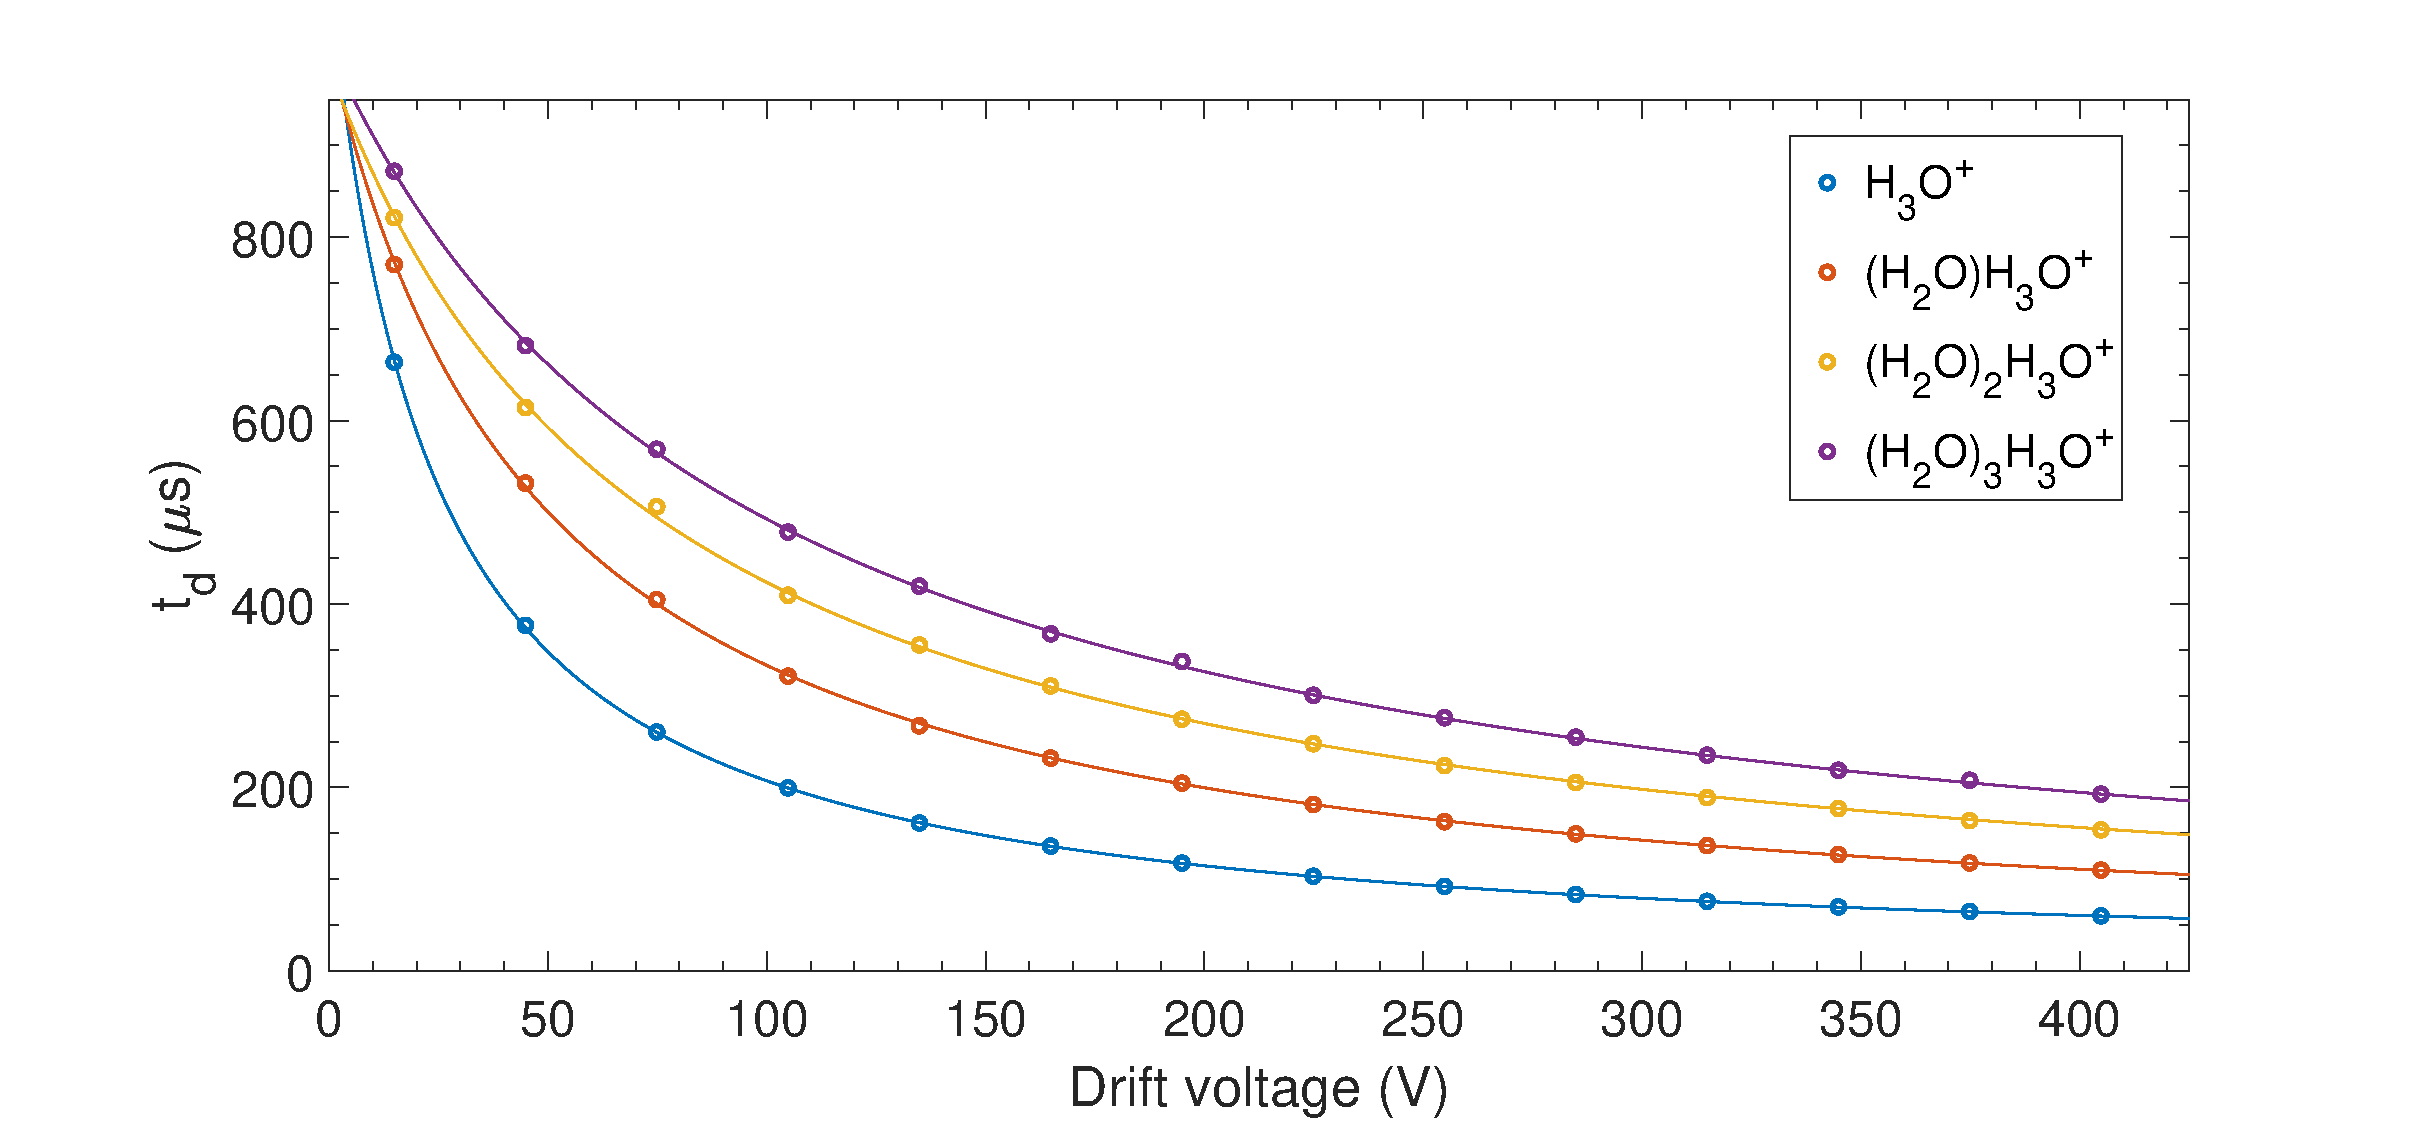
\includegraphics[width=0.9\linewidth]{pics/td.eps}}\\
\bigskip
\sidesubfloat[]{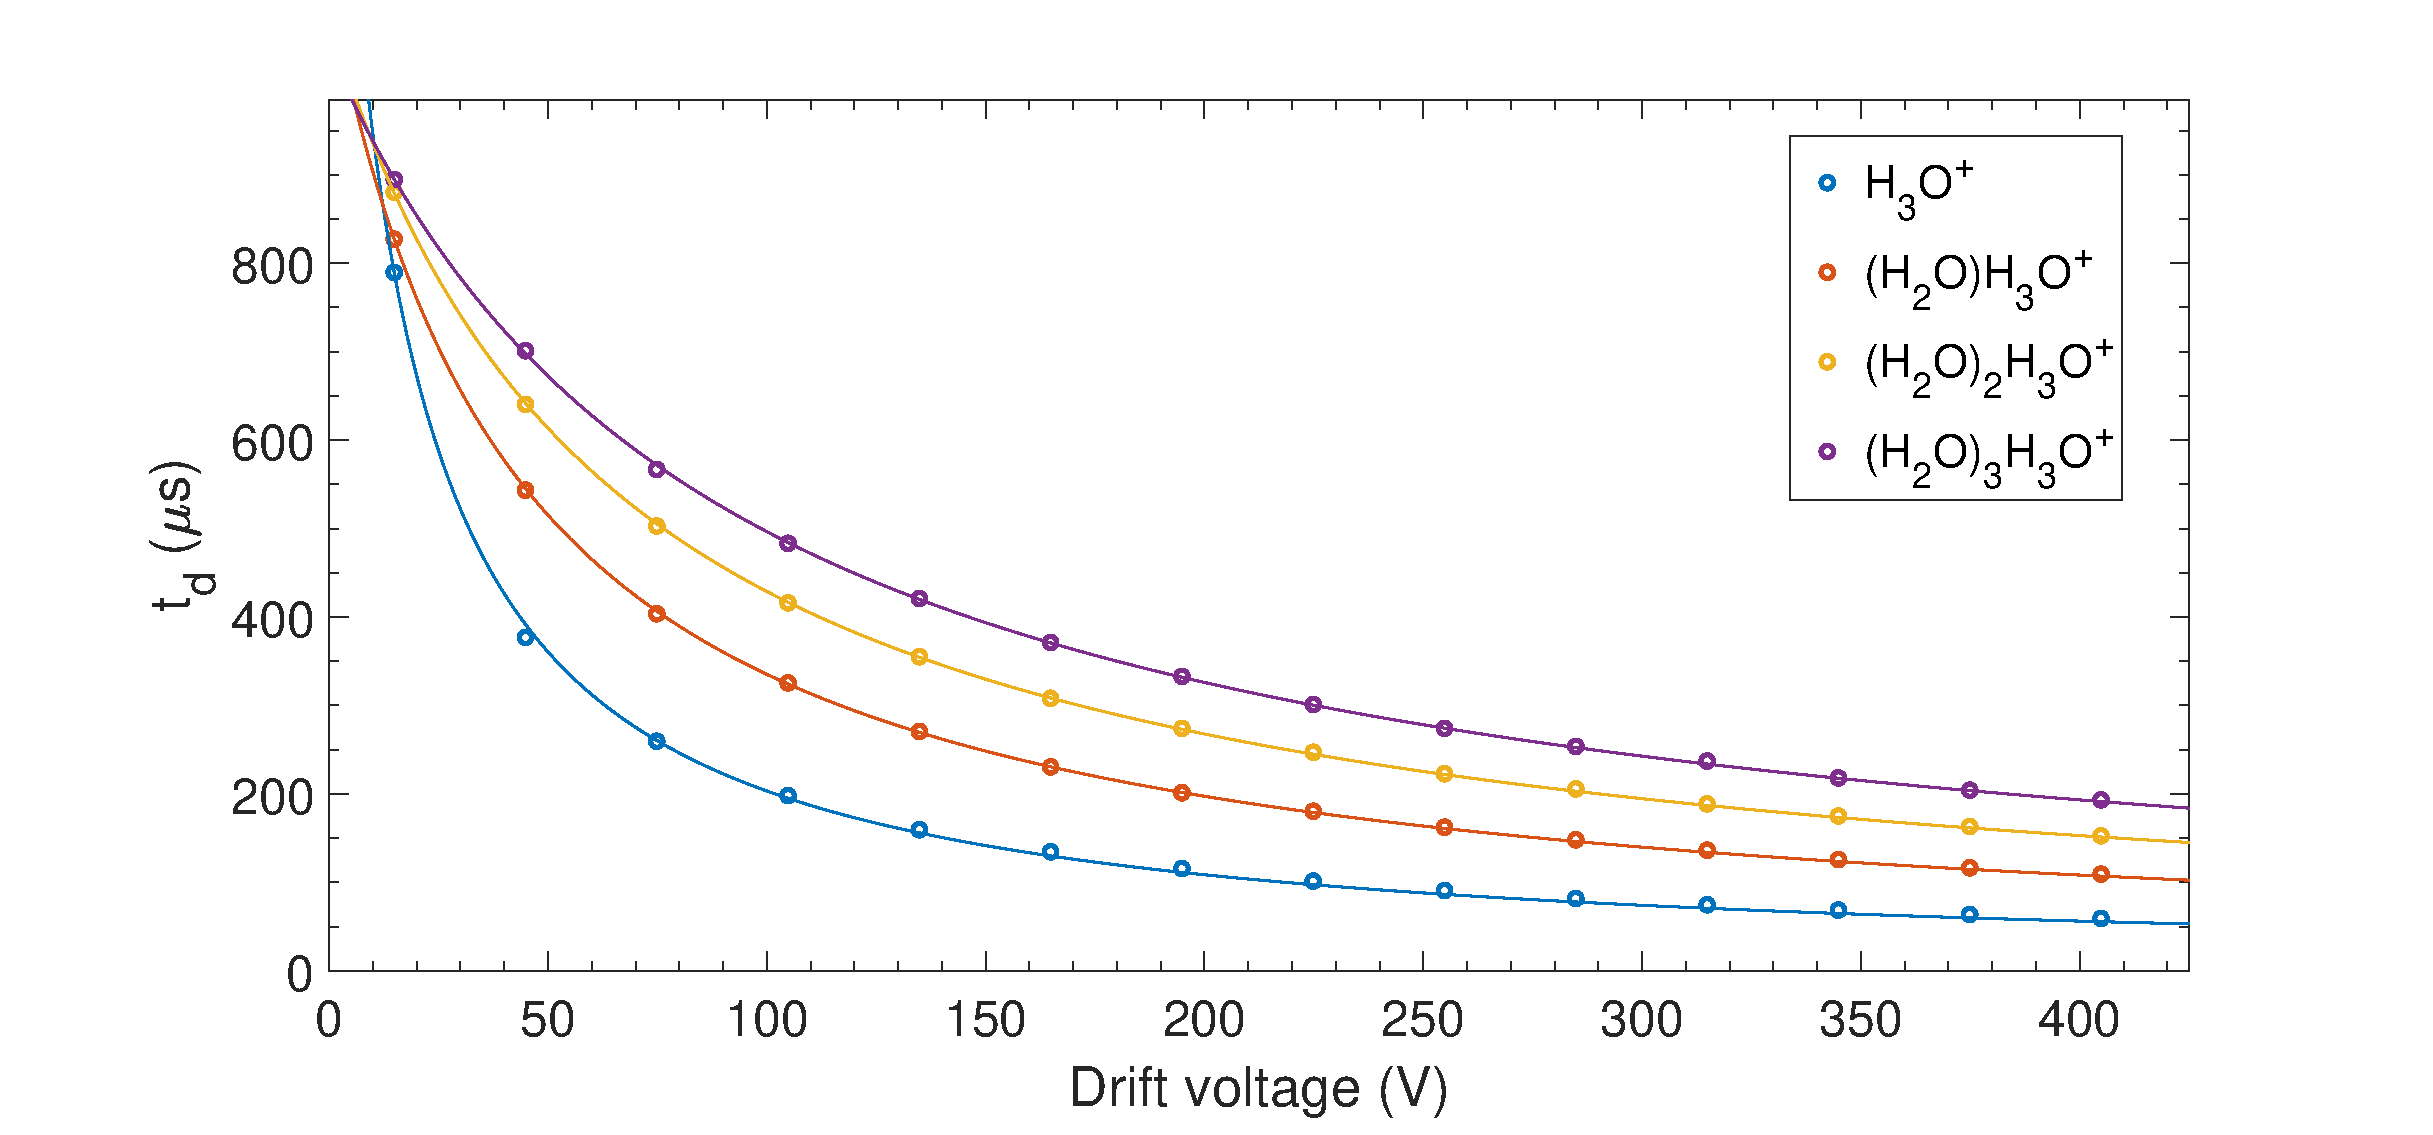
\includegraphics[width=0.9\linewidth]{pics/td_RF.eps}}
\end{center}
\caption{SDS model: Plot of the drift time, t$_d$, as a function of drift voltage for (a) DC mode and (b) RF mode. }\label{fig:td_sds}
\end{figure}



\begin{table}[ht]
\centering
\caption{Coefficients of the fits for the drift time shown in figure \ref{fig:td_sds} using equation \ref{eq:sds_t}.}
\label{tb:tdfit}
\begin{tabular}{llccc}
\toprule
\textbf{Mode}&\textbf{Ion} &\textbf{C$_1$ (V $\mu$s)}	&\textbf{C$_2$   (V)} & \textbf{C$_1$/C$_2$ ($\mu$s)}\\ \midrule 
\ldelim\{{4}{20mm}[\parbox{20mm}{DC mode}]&H$_3$O$^+$&2.56$\times$10$^4$	&23.58&	1085.66		\\
&(H$_2$O)H$_3$O$^+$			&4.98$\times$10$^4$	&49.55&	1005.25		\\
&(H$_2$O)$_2$H$_3$O$^+$		&7.43$\times$10$^4$	&75.41&	985.28		\\
&(H$_2$O)$_3$H$_3$O$^+$		&9.66$\times$10$^4$	&96.00&	1005.73		\\
\bottomrule
\ldelim\{{4}{20mm}[\parbox{20mm}{RF mode}]&H$_3$O$^+$&2.33$\times$10$^4$	&14.67&	1589.64		\\
&(H$_2$O)H$_3$O$^+$			&4.80$\times$10$^4$	&43.13&	1112.45		\\
&(H$_2$O)$_2$H$_3$O$^+$		&7.13$\times$10$^4$	&66.17&	1077.07		\\
&(H$_2$O)$_3$H$_3$O$^+$		&9.49$\times$10$^4$	&91.20&	1041.01		\\
\bottomrule
\end{tabular}
\end{table}


\subsection{Buffer gas velocity}
A = 50 cm$^{2}$, flow = 120 sccm = 2 ssc/s (per second) at 1 mbar. mass flow (mdot) = 2000 scc  mbar/s:
\begin{equation}
v \times A \times P = 2000\, scc \, mbar / s
\end{equation}
v = 40 cm/s = 4$\times$10$^{-3}$ mm/$\mu$s = 0.4 m/s

\newpage
\section{Conclusions and further remarks}
From the results here presented it can be inferred that the higher protonation in RF mode at low drift voltage is a consequence of a long drift time (more time to react) together with the higher collisional energy delivered by the RF field.

Also the hydronium signal in RF mode at low drift voltage is of few tens of thousand counts per second (mz19, not 21; mz 21 is tens of counts). However, when the swab is inserted in the TDU and the analyte is desorbed the hydronium signal is not depleted. The simplest explanation for this is that there is enough hydronium to undergo all the proton transfer without being depleted, but it has a low transmission with this conditions in the reaction.


Further steps: implementation of a clustering/declustering process depending upon the collisional energy (after many collisions, change m/z). It could be something like this: at the beginning of the drift tube only clusters are injected and they dissociate with the collisions. 

Also, the newest version of SIMION allows to implement vectorial fields. This can be used to define a more accurate buffer gas velocity and account for turbulent effects after simulating them with computational flow dynamics (CFD) software.



\subsection{Conclusions: SIMION vs current measurements}
Regarding the current measurements, the current in exit plate monotonously increased with the drift voltage, qualitatively matching the results in my simulations. However, the ion signal (cps) in the detector shows a maximum and then decreases, meaning that there are losses in the transfer lenses region. 


















